\documentclass[journal=langd5,email=true, hyperref=true, keywords=false]{achemso}
\usepackage[utf8]{inputenc}
\usepackage{graphicx}
\usepackage{tabularx}
\usepackage{amsmath}
\usepackage{times}
\DeclareCaptionLabelSeparator{bar}{  \textbar\quad}
\usepackage[labelsep=bar, labelfont=bf]{caption}
\newcommand{\Fig}{Fig.}
\usepackage{units}
\usepackage{txfonts}
\usepackage{xr-hyper}
\usepackage{xcolor}
\usepackage[final]{pdfpages}
\SectionNumbersOn
\mciteErrorOnUnknownfalse       %Clear warning about citings

% \externaldocument[SI-]{SI}


\author{Roman M. Wyss} \affiliation{Soft Materials,
  Department of Materials, Eidgenössische Technische
  Hochschule (ETH) Zürich, Vladimir-Prelog-Weg 1-5, Zürich CH-8093,
  Switzerland.  }
\altaffiliation{R. M. W. and T. T. contributed equally to this work}
\author{Tian Tian} \affiliation{Institute for
  Chemical and Bioengineering Department of Chemistry and Applied
  Biosciences, Eidgenössische Technische Hochschule (ETH) Zürich,
  Vladimir-Prelog-Weg 1-5, Zürich CH-8093, Switzerland.}
\altaffiliation{R. M. W. and T. T. contributed equally to this work}

\author{Khadija Yazda} \affiliation{Nanoscience for Energy Technology and Sustainability,
Department of Mechanical and Process Engineering,
Eidgenössische Technische Hochschule (ETH) Zürich,
Tannenstrasse 3, Zürich CH-8092, Switzerland.}

\author{Hyung Gyu Park} \affiliation{Nanoscience for Energy Technology
  and Sustainability, Department of Mechanical and Process
  Engineering, Eidgenössische Technische Hochschule (ETH) Zürich,
  Tannenstrasse 3, Zürich CH-8092, Switzerland.}
\alsoaffiliation{Mechanical Engineering, Pohang University of Science and
  Technology (POSTECH), 77 Cheongam-ro, Nam-gu, Pohang, Gyeongbuk, 37673,
  Republic of Korea.}
\email{iduserpark@gmail.com}

\author{Chih-Jen Shih}  \affiliation{Institute for
  Chemical and Bioengineering Department of Chemistry and Applied
  Biosciences, Eidgenössische Technische Hochschule (ETH) Zürich,
  Vladimir-Prelog-Weg 1-5, Zürich CH-8093, Switzerland.}
\email{chih-jen.shih@chem.ethz.ch}

\title{Macroscopic Salt Rejection through Electrostatically Gated Nanoporous Graphene}

%%%%%%%%%%%%%%%%%%%%
%Main
%%%%%%%%%%%%%%%%%%%%
\begin{document}
\clearpage{}
\begin{abstract}
  {\normalsize Atomically thin porous graphene is emerging as one of
    the most promising candidates for next-generation membrane
    material owing to the ultrahigh permeation. However, the transport
    selectivity relies on the precise control over pore size and shape
    which considerably compromises the scalability. Here, we study
    electrolyte permeation through a sheet of large-area, porous
    graphene, with relatively large pore sizes of 20$\pm$10
    nanometers. Counterintuitively, a high degree of salt rejection is
    observed by electrostatic gating, reducing the diffusive flux by
    up to one order of magnitude. We systematically investigate the
    effects of salt concentration and species, including developing a
    theory to model the electrolyte diffusion through a nanopore
    drilled in a sheet of gated graphene. The interplay between
    graphene quantum capacitance and the electrical double layer is
    found to selectively modulate the anionic and cationic transport
    paths, creating voltage-dependent electrochemical barriers when
    the pore size is comparable to the Debye length. Our findings
    reveal a new degree of freedom regulating electrolyte permeation
    through porous two-dimensional materials, complementary to the
    pore size design and engineering.}
\end{abstract}

{\begin{flushleft}
\textbf{Teaser}:\\
The quantum capacitance-induced surface potential can stop electrolyte transport through a ``large'' graphene nanopore.
\end{flushleft}
}

%%%%%%%%%%%%%%%%%%%%%%%%%%%%%%
% Main text
%%%%%%%%%%%%%%%%%%%%%%%%%%%%%%
\clearpage{}
\section*{Introduction}
\label{sec:intro}
A central objective in the emerging field of nanofluidics is to
control transport phenomena at nanometer scale to explore new
technological opportunities. The reduction of characteristic
dimensions in nanofluidics gives rise to substantially different
transport properties in comparison to their bulk counterparts
\cite{Schoch_2008}. In nanopores, for example, the effect of
surface-mediated transport becomes dominant when the pore size is
comparable to the characteristic length of diffusion, enabling new
applications such as ionic diodes \cite{Karnik_2007,siwy2002fabrication,vlassiouk2007nanofluidic}, field-effect
transistors \cite{Nam_2009}, desalination \cite{Heiranian_2015}, and
nanopore-based DNA sequencing \cite{Heerema_2016,Garaj_2013}. Porous,
atomically thin two-dimensional (2D) materials, such as graphene, are
emerging as ideal membrane materials due to the ultimate permeation
\cite{Suk_2010,Jiang_2009,Celebi_2014,Koenig_2012,Drahushuk_2012}. Early
research has suggested that using a sheet of nanoporous graphene can
act as a desalination membrane by having the pore sizes smaller than
the hydrated radii ($\sim$1 nm), thereby hindering ion passage without
losing water permeability
\cite{Cohen_Tanugi_2012,Suk_2014,Cohen_Tanugi_2014,Cohen_Tanugi_2015,O_Hern_2014,O_Hern_2015,Surwade_2015,Walker_2017,Ghosh_2018}. Nevertheless,
in practice, the fabrication of subnanometer porous 2D membranes over
a large area with atomic precision remains technically challenging, 
limiting the effective separation
  % or demanding leak-sealing mechanism such as interfacial polymerization
\cite{Suk_2014,Rollings_2016,O_Hern_2012,Wang_2017}. Moreover, a small
portion of excessively large pores or tears can significantly diminish
salt rejection. Regarding these issues, we have previously developed a
highly-scalable technique to fabricate uniformly-distributed nanopores
(sub-20 to 50 nm) over wafer-scale graphene samples
\cite{Choi_2018}. A major step towards its real-world desalination and
separation applications, would be to develop methodology that allow
appreciable selectivity of nanoporous 2D membrane with pore size even
larger than the hydration radii. A number of recent reports have
explored the effect of surface charges on the selectivity of ion
transport through graphene nanopores, as a consequence of the
electrostatic interactions between solvated ions and the charged
functional groups attached on graphene, indicating that even large
pores ($>$ 30nm) can be ion selective
\cite{Rollings_2016,Surwade_2014}. However, it remains controversial
that if the surface charges can result in a degree of salt rejection,
as the surface charge and potential cannot be precisely quantified and
are sensitive to the surroundings as well as the history of chemical
treatment \cite{Li_2008}. There remains a lack of fundamental
understanding of the interactions between the charged 2D nanopores and
the electrolyte solution, { especially in regard of controlled ion
  transport modulation}.

In this report, we investigate electrolyte permeation through graphene
nanopores that are significantly larger than the hydration radii. We
model the surface potential by taking into account the elementary
electronic properties of graphene and demonstrate that a high degree
of salt rejection could be achieved by both pore sizing and
electrostatic gating.

\section*{Results and discussions}
\label{sec:res}

\subsection*{Free diffusion through porous graphene}
\label{sec:res-1}

Fig. \ref{fig:1}a depicts the experimental setup characterizing
ionic diffusion through a sheet of double layer porous graphene
(PG). Two reservoirs, namely the high-concentration reservoir (HCR)
containing electrolyte solution with molar concentration $c_0$, and
the low-concentration reservoir (LCR) containing de-ionized (DI)
water, are separated by a PG membrane supported by a polycarbonate
track-etched (PCTE) film. Magnetic stirrers are used to minimize the
effects of external concentration polarization, and a conductivity
probe is placed in the LCR to monitor the ionic concentration as a
function of time. The membrane is attached to a piece of copper tape
connected to a voltage source applying an electrical bias
$V_{\mathrm{G}}$, with the LCR grounded (Fig. \ref{fig:1}a
inset). We fabricated the PCTE-supported PG as schematically shown in
Fig. \ref{fig:1}b, using the protocol developed by our group
\cite{Choi_2018}, which  enables formation of uniformly-distributed graphene  nanopores over large area up
 to 25 cm$^{2}$ (details see Supplementary Section
\ref{sec:exp}). The normally distributed, circular pores with pore
diameters of 20$\pm$10 nm and a pore density of
1.25$\pm$0.25$\times$10$^{10}$ cm$^{-2}$ (Fig. \ref{fig:1}c inset)
over a large area were perforated on graphene.  By optimizing the
subsequent transfer process, a high surface coverage ($>$ 98\%) of PG
on PCTE was obtained (Fig. \ref{fig:1}c), allowing reliable
characterization of the ion transport behavior (details see
Supplementary Section \ref{sec:exp}).  The system presented here
allows us to systematically investigate the diffusive flux of ions
across a sheet of PG, $\boldsymbol{J}$, driven by the gradient of
electrochemical potential in the electrolyte medium.

First, the control experiments were carried out by measuring the ionic
diffusion of seven salt species, including KCl, NaCl, LiCl,
K$_{2}$SO$_{4}$, MgSO$_{4}$, CaCl$_{2}$ and K$_{3}$[Fe(CN)$_{6}$],
through the bare PCTE membrane at $c_{0}$ = 0.1 mM. As the diffusive
flux is comparably small, the conductivity increases linearly with
time in the LCR (e.g. Fig. \ref{fig:2}a) within the measurement
duration (1 h), suggesting the concentration gradient across the
membrane remains constant. The diffusive fluxes (blue bars in Fig.
\ref{fig:2}b) of different salts were obtained by converting the
conductivity-time profiles using calibration curves (Supplementary
Section \ref{sec:measure}). The theoretical diffusive fluxes
through PCTE are obtained based on the assumption that the membrane
consists of cylindrical pores with uniform diameter and a low
tortuosity $\tau$ of $\sim{}$1.2 \cite{O_Hern_2012}:
\begin{equation}
  \label{eq:j-pcte}
  \boldsymbol{J}_{\mathrm{PCTE}} = \frac{\pi r_{\mathrm{PCTE}}^{2} N_{\mathrm{p}} D_{\mathrm{\pm}} \Delta c}{L \tau}
\end{equation}
{where $r_{\mathrm{PCTE}}$ (= \unit[200]{nm}) is the PCTE pore radius, $N_{\mathrm{p}}$  (= \unit[$1.5\cdot10^{12}$]{m$^{-2}$}) is
numbers of pore per area, $D_{\mathrm{\pm}}$ is the salt diffusivity
(average of cation and anion diffusivity), $\Delta c$ is the bulk
concentration difference between two reservoirs, i.e.,
$\Delta c \sim c_{0}$ and $L$ (= \unit[24]{$\muup$m}) is the thickness of the PCTE membrane.
By using the salt diffusivity values (Supplementary Table
\ref{tab:diff}), the calculated diffusive fluxes (red bars in
Fig. \ref{fig:2}b) show reasonable agreement with the experimental
values.}

Next, we carried out the same experiments using the PG-covered PCTE
membrane (PG-PCTE), without electrostatic gating. The measured
diffusive flux values, $\boldsymbol{J}_{\mathrm{PG0}}$ (green bars in
Fig. \ref{fig:2}b), remain at the same order of magnitude compared
with those of bare PCTE membrane, suggesting that the transport
resistance of PCTE $R_{\mathrm{PCTE}}$, is dominant over that of PG
without gating, $R_{\mathrm{G}}^{0}$. Using a simple circuit model, we
estimate the ratio $\delta$ between $R_{\mathrm{G}}^{0}$ and
$R_{\mathrm{PCTE}}$, i.e.,
$\delta = R_{\mathrm{PCTE}}/R_{\mathrm{G}}^{0}$, to be $\sim$2.2,
which is in good agreement with the value derived from the
experimental data in Fig. \ref{fig:2}b (details see Supplementary
Section \ref{sec:R-model}).
% \todo[inline]{Make sure that the
  % values used are correct.}


\subsection*{Salt rejection induced by electrostatic gating}
\label{sec:res-2}

We next discuss the effects of electrostatic gating on graphene. 
{ Electrostatic gating has been employed previously to alter the 
ion permeation through nanoporous structures. For example, an applied bias on a mesoporous 
carbon membrane, having pores of $<$\unit[5]{nm}, allows to stop the 
ion flux once the Debye length of the solution approaches the pore size \cite{Surwade_2014}. 
Similar experiments using nanoporous gold membranes, however, find that the cation and anion 
transport is enhanced upon applying a bias \cite{mccurry2017electrolyte}. While the former behavior 
was ascribed to the depletion of the channel from ions upon gating, the latter was a result of enhanced transport
by dominating drift currents.}


In order to investigate the behavior in more detail, the ``three-interval'' method, which has been used
in controlling the membrane potential in mesoporous carbon membranes
\cite{Surwade_2014}, is adopted here. Fig. \ref{fig:2}a
illustratively represents how the measured conductivity evolves with
time. Specifically, in the first interval, the gate voltage source is
turned off and the conductivity probe is on, allowing us to obtain the
conductivity-time profile with an average slope $s_{1}$ that
corresponds to the diffusive flux across the PG-PCTE membrane. In the
second interval, a voltage $V_{\mathrm{G}}$ is applied to the membrane
after turning off the conductivity probe, followed by the third
interval $s_{3}$, in which the conductivity probe is turned on again
to give the corresponding slope. A control experiment was performed to
ensure the copper tape was not in direct contact with the ionic
solution (Supplementary Section \ref{sec:copper}). The slope
corresponding to the second interval $s_{2}$, as the conductivity
probe is off, is determined by linear interpolation of the
conductivities from the endpoint of interval 1 to the starting point
of interval 3. A decrease of slope observed in interval 2 indicates
that the total flux through PG-PCTE is reduced upon gating (i.e. salt
penetration through the PG pores is hindered). We define such
experimentally measured reduction rate as $\eta$, which is equivalent
to the decrease of total diffusive flux through PG-PCTE as follows:
\begin{equation}
  \label{eq:rejection}
  \eta = \frac{\bar{s} - s_{2}}{\bar{s}} = \frac{\boldsymbol{J}_{\mathrm{PG0}}
    - \boldsymbol{J}_{\mathrm{PG}}(V_{\mathrm{G}})}{\boldsymbol{J}_{\mathrm{PG0}}}
\end{equation}
where $\bar{s}$ is the average slope of $s_{1}$ and $s_{3}$, namely
$(s_{1} + s_{3})/2$, and
$\boldsymbol{J}_{\mathrm{PG}}(V_{\mathrm{G}})$ is the diffusive flux
across the PTCE-supported PG double layer as a function of
$V_{\mathrm{G}}$. Since graphene and PCTE membranes effectively form a
transport system with series diffusive resistance $R_{\mathrm{G}}$
(tunable by $V_{\mathrm{G}}$) and $R_{\mathrm{PCTE}}$ (independent of
$V_{\mathrm{G}}$), respectively, we define the effective degree of
salt rejection from bare PG, $\xi$, as a function of $V_{\mathrm{G}}$ (
details see Supplementary Section \ref{sec:R-model}) as:
\begin{equation}
\label{eq:xi-def}
\xi = 1 - \frac{R_{\mathrm{G}}(V_{\mathrm{G}}=0)}{R_{\mathrm{G}}(V_{\mathrm{G}})} = \frac{(\delta+1) \eta}{\delta \eta + 1}
\end{equation}
The factor $\xi$ is a reliable and stable measure of salt rejection
through the PG membrane itself upon gating, as the salt species and
initial conditions may induce a degree of measurement uncertainty
between different samples. Note that the $\xi=1$ limit represents
perfect salt rejection in which
$R_{\mathrm{G}}(V_{\mathrm{G}}) \to \infty$. On the contrary $\xi=0$
indicates $R_{\mathrm{G}}$ remains unchanged with $V_{\mathrm{G}}$.

Using 0.1 mM KCl solution in HCR, we obtained $\xi$ as a function of
$V_{\mathrm{G}}$ within $\pm1.25$ V, before triggering the
electrochemical reactions (Fig. \ref{fig:2}c). We observe an
asymmetric dependence of $\xi$ with respect to $V_{\mathrm{G}}$, with
a higher degree of salt rejection for $V_{\mathrm{G}}>0$. where
positive carriers (holes) are induced in graphene. We notice that an
increase of $\xi$, or a decrease of diffusive flux through PG with
$V_{\mathrm{G}}$, shows an inverse trend compared with those
observed in ionic field effect transistors (IFETs) in which the
diffusive flux increases with the gate voltage
\cite{Nam_2009,Cheng_2018}. A further increase of the KCl
concentration $c_{0}$ influences the obtainable degree of salt
rejection. 
We note small negative $\xi$ values (corresponding to reduced transport resistance) at $V_{\mathrm{G}} \sim{}$ -0.5 V
likely caused by (i) offset of the charge neutral point (CNP) of graphene is from $V_{\mathrm{G}}$ = 0 and (ii) experimental uncertainty.
Nevetherless, significant salt rejection is observed when $V_{\mathrm{G}}>$ 0.5 V.
The $\xi$ values measured at $V_{\mathrm{G}}$ = 1.25 V,
$\xi_{\mathrm{max}}$, as a function of $c_{0}$ from 10$^{-4}$ to
10$^{-2}$ M KCl (see Supplementary Section \ref{sec:debye}) exhibit
a power law dependency (Fig. \ref{fig:2}d). The
$\xi_{\mathrm{max}}-c_{0}$ relation can be nicely fitted by a power
law function following
$\xi_{\mathrm{max}} c_{0}^{0.52} = \mathrm{constant}$. As the Debye
length in solution, $\lambda_{\mathrm{D}}$, is inversely proportional
to $c^{0.5}$, we infer that the $V_{\mathrm{G}}$-induced salt
rejection originates from the modulation of the electrical double
layer (EDL), as will be discussed later.

\subsection*{Self-consistent ion transport theory}
\label{sec:theory}

In order to quantitatively understand the observed $V_{\mathrm{G}}$
dependence, we develop a theory to model the coupling of graphene's
elementary transport properties and EDL, in order to quantify the
ionic transport through a graphene nanopore. Under the assumption that
the time scale for the bulk concentration change is significantly
longer than that of ionic diffusion, the pseudo-steady state
approximation holds. Accordingly, the steady-state Nernst-Planck
equation describing the ionic transport in an electrolyte solution is
given by \cite{MacGillivray_1968}:
\begin{equation}
  \label{eq:pnp}
  \nabla \cdot \boldsymbol{J}_{i} = -\nabla \cdot (\frac{D_{i}}{k_{\mathrm{B}}T} c_{i} N_{\mathrm{A}} \nabla \mu_{i}) = 0
\end{equation}
where $\boldsymbol{J}$ is the mass flux, subscript \textit{i}
corresponds to the ionic species (anion or cation), $D$ is the diffusivity,
$k_{\mathrm{B}}$ is the Boltzmann constant, $T$ is temperature, $c$ is
the molar concentration, $N_{\mathrm{A}}$ is the Avogadro constant,
and $\mu_{i}$ is the electrochemical potential. Under the assumption
of ideal solution, it follows \cite{Kilic_2007}:
\begin{equation}
  \label{eq:mu}
  \nabla \mu_{i} = k_{\mathrm{B}} T \nabla \ln x_{i} + z_{i} e \nabla \psi
\end{equation}
 $x$ is the molar fraction in solution, $z$ is the ionic valence,
$e$ is the unit charge, and $\psi$ is the electric potential. On the
other hand, the Poisson equation describing the electric potential
distribution is given by:
\begin{equation}
  \label{eq:poisson}
  \nabla \cdot (\varepsilon_{\mathrm{m}} \varepsilon_{0} \nabla \psi)
  =
  - N_{\mathrm{A}} e \sum_{i} c_{i} z_{i}
\end{equation}
where $\varepsilon_{\mathrm{m}}$ is the relative permittivity of
individual materials in the system, including water and the internal
Stern layer\cite{Tian_2017}, and
$\varepsilon_{0}$ is the vacuum permittivity. When applying
$V_{\mathrm{G}}$ to graphene adjacent to the electrolyte solution,
charges (electrons or holes) are induced in graphene; the
electroneutrality of the entire system suggests:
\begin{equation}
  \label{eq:electro-neutral}
  \sigma_{\mathrm{G}} S_{\mathrm{G}} + \sum_{i} \int_{\Omega} z_{i} c_{i} N_{\mathrm{A}} e \mathrm{d}^{3} \Omega= 0
\end{equation}
where $\sigma_{\mathrm{G}}$ is the charge density in graphene,
$S_{\mathrm{G}}$ is the total area of graphene, and $\Omega$
corresponds to the entire volumetric domain of electrolyte
solution. Note that the graphene surface potential,
$\psi_{\mathrm{G}}$, is not equivalent to $V_{\mathrm{G}}$ due to
change of graphene's work function upon charging, known as the
graphene quantum capacitance effect\cite{Xia_2009} (Fig.
\ref{fig:3}a) following:
\begin{equation}
  \label{eq:Vg}
  V_{\mathrm{G}} = \Delta \phi_{\mathrm{G}} + \psi_{\mathrm{G}}
\end{equation}
where
$\Delta \phi_{\mathrm{G}} = \phi_{\mathrm{G}}(V_{\mathrm{g}}) -
\phi_{\mathrm{G}}(V_{\mathrm{g}}=0)$ is the change of graphene’s work
function. The properties of the PG samples fabricated is close to
intrinsic graphene, with charge density at $V_{\mathrm{G}}=0$ measured
to be 1.4$\times$10$^{11}$ \textit{e}$\cdot$cm$^{-2}$, corresponding
to a work function difference of 48 meV from graphene's Dirac point
(details see Supplementary Section \ref{sec:charge-dens}), much
smaller than the $\Delta \phi_{\mathrm{G}}$ induced by gating.
Therefore, we adopt the simplification that the charge neutrality point
of graphene coincides with the Dirac point at $V_{\mathrm{G}}$ =
0. The elementary electronic properties of graphene give:
\begin{equation}
  \label{eq:delta-phiG}
  \Delta \phi_{\mathrm{G}} = \mathrm{sign}(\sigma_{\mathrm{G}}) \frac{\hbar v_{\mathrm{F}}}{e}
  \sqrt{\frac{\pi |\sigma_{\mathrm{G}}|}{e}}
\end{equation}
where $\hbar$ is the reduced Planck constant, and
$v_{\mathrm{F}}=1.1\times10^{6}$ m$\cdot$s$^{-1}$ is the Fermi
velocity of graphene \cite{Tian_2016}.  Note that the PG film
fabricated experimentally is double-layer turbostratic (randomly
aligned) graphene, in which we assume the
$\Delta \phi_{\mathrm{G}} - \sigma_{\mathrm{G}}$ dependence follows
Eq. \eqref{eq:delta-phiG}. The influence of polymer residue on the
surface of graphene is not considered in the current theory due to:
(i) insulating polymer residues do not respond to the gate voltage and
(ii) the thickness of the polymer residue is minimal after the thermal
annealing process. The theory proposed here was solved
self-consistently by discretizing
Eqs. \eqref{eq:pnp}-\eqref{eq:poisson} using the finite-element method
(FEM), in which the graphene surface potential is coupled with
Eqs. \eqref{eq:electro-neutral}-\eqref{eq:delta-phiG} that were solved
simultaneously to reach convergent numerical solutions of
$\sigma_{\mathrm{G}}$ and $\psi_{\mathrm{G}}$ for a given
$V_{\mathrm{G}}$. Clearly, the above model yields symmetric
characteristics for $\sigma_{\mathrm{G}}$ and $\psi_{\mathrm{G}}$ with
respect to $V_{\mathrm{G}}$ due to the symmetric band structure of
graphene (Eq. \eqref{eq:delta-phiG}). However, for graphene
synthesized by chemical vapor deposition (CVD) used in our
experiments, it is well-recognized that the electron traps are
inherently introduced during synthesis and patterning
\cite{Dean_2010}, effectively reducing the charge density and surface
potential on graphene $V_{\mathrm{G}}<0$ (Supplementary Fig.
\ref{fig:trap}), which is related to the fact that observed $\xi$ is
much lower within the $V_{\mathrm{G}}<0$ regime in Fig.
\ref{fig:2}c. With the nonideality in mind, hereafter, we compare the
calculations and experiments in the regime of $V_{\mathrm{G}}>0$. For
example, Fig. \ref{fig:3}b presents the calculated
$\sigma_{\mathrm{G}}$ and $\psi_{\mathrm{G}}$ as a function of
$V_{\mathrm{G}}$ considering the ionic diffusion through a single 20
nm-diameter nanopore drilled on a sheet of semi-infinite double layer
graphene that separates HCR containing KCl solution at $c_{0}$ = 0.1
mM, and LCR at $c_{0}/10$ in axisymmetric coordinates (details see
Supplementary Section \ref{sec:numer}). Indeed, the interplay between
graphene quantum capacitance and the EDL significantly reduces the
graphene surface potential $\psi_{\mathrm{G}}$ to $\sim$0.3 V at
$V_{\mathrm{G}}$ = 1.25 V, corresponding a surface charge density
$\sigma_{\mathrm{G}}$ of $\sim$0.08 C$\cdot$m$^{-2}$. Note that as we
mentioned earlier, an important merit of the 2D nanopore system
considered here is that the surface charge density can be precisely
determined and controlled, rather than being treated as a fitting
parameter as in most of the 2D nanopore literature
(e.g. Ref. \citenum{Rollings_2016}). In addition, we anticipate that
the gate-controlled ionic transport can also be achieved by replacing
graphene with other nanoporous conducting 2D materials, while they are
less practical due to the narrower operational window of gate voltage
required to achieve the same level of salt rejection. This is because
graphene has the smallest quantum capacitance (near the Dirac point)
among all known 2D materials \cite{Tian_2016}.

\subsection*{Salt rejection mechanism}
\label{sec:mechanism}

The numerical procedure described above allows us to resolve the
concentration and electric potential profiles near a graphene
nanopore for a given $V_{\mathrm{G}}$. Since the ionic flux is driven
by both $\psi$ and $c$ fields (see Eq. \eqref{eq:pnp} and \eqref{eq:mu}),
we focus on the electrochemical potential $\mu_{i}$, which represents
the combined driving force, to reveal its dependence on the applied
$V_{\mathrm{G}}$. Following the same system considered in Fig.
\ref{fig:3}b, the calculated axisymmetric electric potential $\psi$
and the relative electrochemical potentials,
$\Delta \mu_{\mathrm{K^{+}}}$ and $\Delta \mu_{\mathrm{Cl^{-}}}$, for
$V_{\mathrm{G}}$ = 0.75 V are shown in Fig. \ref{fig:4}a and
\ref{fig:4}b, respectively. The reference point of the electrochemical
potentials is set at the bulk phase in the HCR. As expected, the
electric potential reaches the maximum at the graphene surface (with
$\psi_{\mathrm{G}}$ of $\sim$100 mV) and decays towards the bulk
solution phase, forming an EDL surrounding the graphene surface. Since
the Debye length $\lambda_{\mathrm{D}}$ is comparable to the
pore radius $r_{\mathrm{G}}$, the electric potential at the nanopore
center remains at $\sim$25 mV, comparable to the thermal energy at
room temperature ($k_{\mathrm{B}}T$ = 26 meV). Consequently, it is
evident that the potential barrier is sufficient to modulate the
diffusive flux.

We further reveal the cation and anion transport pathways by looking
into their electrochemical potentials (Fig. \ref{fig:4}b). By
increasing $V_{\mathrm{G}}$, a more positive $\psi_{\mathrm{G}}$ on
graphene surface reduces the cation concentration at the pore edge due
to the electrostatic interactions, thereby increasing its
concentration gradient at the pore center. On the other hand, the
anion concentration near the pore edge increases exponentially, such
that the concentration gradient at the pore center becomes small (see
{ Supplementary Section \ref{sec:conc}, Supplementary
Figs. \ref{fig:conc} and \ref{fig:conc-r}}).
{
Although the surface
concentration of anions is enhanced by $\sim{}$30 times, it is sill
much smaller than the saturated surface adsorption density, and the
bulk diffusivity used in the Nernst-Planck equation still holds.  We
also observe that $\Delta \mu_{+}$ is dominated by the concentration,
while $\Delta \mu_{-}$ is much less than $\Delta \mu_{+}$ due to the
balance between the diffusion and drift potentials (see Supplementary
Section \ref{sec:conc}, Supplementary Figs.  \ref{fig:potential}
and \ref{fig:flux})}. 
The observations confirm the distinct ionic
transport pathways upon applying a positive $V_{\mathrm{G}}$: pore
center for cations and pore edge for anions. Fig. \ref{fig:4}c
presents the calculated \textit{z}-component of the cation and anion
fluxes through the pore at the graphene plane (z = 0),
$\boldsymbol{J}_{z}$ ,as a function of the normalized radius,
$r/r_{\mathrm{G}}$ , where $r$ is the radial coordinate and
$r_{\mathrm{G}}$ is the pore radius, at different $V_{\mathrm{G}}$
values. Note that $\boldsymbol{J}_{z}$ is negative because the LCR is
placed at z$<$0 in the simulation box. At $V_{\mathrm{G}}$ = 0 (pure
diffusion), the anion and cation flux profiles are identical, with a
higher flux near the pore edge, which is expected, as the
concentration gradient is higher. By gradually increasing
$V_{\mathrm{G}}$, both fluxes are reduced throughout the pore, while
the degree of reduction is more pronounced at the pore edge for the
cation, and at the pore center for the anion, following the scenarios
we discussed above. Accordingly, the integrated fluxes across the
pore, $|\boldsymbol{J}_{z}|$, are reduced with $V_{\mathrm{G}}$
(Fig. \ref{fig:4}d). A total flux reduction of $\sim$90\% is
predicted. Another interesting finding here is that, by increasing
$V_{\mathrm{G}}$, the nanopore transport preferentially allows cations
over anions, or in other words, the anion flux is more reduced with
$V_{\mathrm{G}}$ (see Fig. \ref{fig:4}c), known as the ion
selectivity of graphene nanopore \cite{Rollings_2016}. In our setup,
the imbalance between cation and anion fluxes near the graphene
nanopore is compensated by the EDL formation at the counter-electrode
in LCR, which maintains the electroneutrality of the system. Notably,
since atomically thin graphene samples are used, the mechanism of salt
rejection is clearly distinct from that in capacitive deionization
\cite{Biesheuvel_2010}, where electrodes with large surface area are
required. 
{
More detailed discussion about the selective ionic pathways
upon gating can be found in Supplementary Section \ref{sec:conc}.}

The above mechanistic findings, nevertheless, do not fully clarify the
experimentally observed reduction of diffusive flux upon
gating. Indeed, the same physical mechanism also governs 
the 
{ diode-like ionic
transport through an IFET  \cite{Nam_2009,Lee_2015,Feng_2016}
or a nanoporous metal membrane \cite{mccurry2017electrolyte}},
in which a nonzero electric potential at
the nanopore center usually results in an increase of ionic
conductivity. To this end, we
further increased the graphene surface potential $\psi_{\mathrm{G}}$
considering the same system (details see Supplementary Section
\ref{sec:conc}). Intriguingly, by increasing
$\psi_{\mathrm{G}}$ larger than 400 mV, the ionic flux starts to
increase, reversing the trend observed at the low $\psi_{\mathrm{G}}$
regime, due to scenarios that (i) the drift flux become dominant over diffusion flux
and (ii) the concentration near the pore edge (preferred path) greatly
increases (details see Supplementary Section \ref{sec:conc},
Supplementary Figs. \ref{fig:reverse} and
\ref{fig:large-V}). This level of $\psi_{\mathrm{G}}$ cannot be
reached experimentally in graphene membrane, as this requires a
$V_{\mathrm{G}}$ larger than 2.0 V, which triggers the electrochemical
reactions \cite{Toh_2011}. On the other hand, in an IFET, the electric
potential on the pore wall is considerably higher, equivalent to
$V_{\mathrm{G}}$ due to the metallic nature of gate electrode (having
an infinitely-large quantum capacitance). We therefore conclude that
the quantum capacitance-induced nonlinear damping in the surface
potential results in the observed salt rejection.  Following the above
discussions, we further investigate the physical limits for the biased
graphene nanopores. Specifically, the salt rejection characteristics
are controlled by: (i) the overlap of EDL inside the nanopore,
essentially controlled by two length scales of $\lambda_{\mathrm{D}}$
and $r_{\mathrm{G}}$, and (ii) the graphene surface potential
$\psi_{\mathrm{G}}$ controlled by $V_{\mathrm{G}}$ following
Eq. \eqref{eq:Vg}. To this end, we calculate $\psi_{\mathrm{G}}$ as a
function of $\lambda_{\mathrm{D}} / r_{\mathrm{G}}$ and
$V_{\mathrm{G}}$ (Fig. \ref{fig:5}a). Clearly, when the bulk
concentration $c_{0}$ increases, a higher $V_{\mathrm{G}}$ is required
to reach the same level of $\psi_{\mathrm{G}}$. Consequently, as
revealed in Fig. \ref{fig:5}b, the calculated salt rejection factor
$\xi$ increases with both $\lambda_{\mathrm{D}} / r_{\mathrm{G}}$ and
$V_{\mathrm{G}}$, in line with the experimentally observed
$\xi - c_{0}$ dependence. We also find the overall trends for
$\psi_{\mathrm{G}}$ and $\xi$ with respect to
$\lambda_{\mathrm{D}}/r_{\mathrm{G}}$ and $V_{\mathrm{G}}$ are very
similar. More importantly, based on our theoretical prediction, with
$V_{\mathrm{G}}$ = 1.25 V and $\lambda_{\mathrm{D}} / r_{\mathrm{G}}$
= { 2.0},
a high value of $\xi$ up to $\sim$0.95 can be achieved.  We
notice that although the above analysis suggests a salt rejection up
to 1 may be achived by further reducing the pore size (i.e. increasing
the $\lambda_{\mathrm{D}}/r_{\mathrm{G}}$ ratio), our theory, derived
from on the macroscopic transport equations by treating ions as
zero-volume charges, may not be valid when $r_{\mathrm{G}}<$ 5
nm\cite{Jain_2015}. In addition, the specific ion-graphene
interactions \cite{Rollings_2016} are not taken into account. Advanced
theoretical frameworks that bridge continuum and molecular models are
required to elucidate electrolyte transport approaching the small pore
limit. 
{
We notice that the calculations in Figs. \ref{fig:4} and \ref{fig:5} 
are based on the setup  of ionic transport through a single nanopore.
In order to mimic the experimental conditions, 
calculations were carried out by considering the pore size distribution in Fig. \ref{fig:1}c inset. 
Under the assumption that the interpore distance is significantly larger than the Debye length,
the overall salt rejection $\xi$ is
estimated by the linear combination of the salt rejection 
$\xi_{r_i}$ 
from individual pores with radius $r_i$ given by:
\begin{equation}
\label{eq:rejection-comb}
\xi = \sum_{r_{i}} \xi_{r_{i}} w_{r_{i}}
\end{equation}
where
$w_{r_{i}} = x_{r_{i}} r_{i}^{2} / \sum_{r_{i}} x_{r_{i}} r_{i}^{2} $
is the contribution factor from pores with radius $r_{i}$, and
$x_{r_{i}}$ is the fraction of pores with radius $r_{i}$ (details see
Supplementary Section \ref{sec:pore-dist}). Combining
Eq. \ref{eq:rejection-comb} and Fig. \ref{fig:5}b, the calculated salt
rejection is reduced to $\sim{}$ 80\% of that from the single-pore
calculation of a 20 nm nanopore when $c_{0}$ = 0.1 mM (Supplementary
Fig.  \ref{fig:simple-rect-pore}). Consider the existence of large
pores with diameter up to 60 nm, such degree of salt rejection is
still appreciable, which is ascribed to the nonlinear dependency of
$\xi$ on $\lambda_{\mathrm{D}} / r_{\mathrm{G}}$ and $V_{\mathrm{G}}$
(details see Supplementary Section \ref{sec:pore-dist}).}  From our
analysis, it is also clear that reducing the average pore size is critical
to overcome the low salt rejection at higher concentrations, which may
hopefully be achieved with relevant fabrication techniques.

\subsection*{Effects of salt species}
\label{sec:salts}

Finally, we examine other salt species and compare the degree of salt
rejection between experiments and simulations. Fig. \ref{fig:6}a
presents the measured salt rejection $\xi$ as a function of
$V_{\mathrm{G}}$ at $c_{0}$ = 0.1 mM, for the seven salt species
considered here, including NaCl, LiCl, KCl, MgSO$_{4}$, CaCl$_{2}$,
K$_{2}$SO$_{4}$, and K$_{3}$[Fe(CN)$_{6}$] (details see Supplementary
Section \ref{sec:salts}). Similar to the KCl system discussed
earlier, the salt rejection is more pronounced in the positive
$V_{\mathrm{G}}$ regime. 
% { The negative $\eta$ values, observed for certain salts or applied $V_{\mathrm{G}}$, respectively, would actually
% indicate that the flow in enhanced upon biasing the membrane. While such behavior is not uncommon in gating systems, we cannot conclude unambiguously if the effect is significant or rather within the measurement uncertainty of the system. Furthermore, as the definition of $\xi$ based on $\delta$ is only valid for positive $\eta$, the discussion is hence limited to $V_{\mathrm{G}}$ $>$ 0.}
The degree of salt rejection deceases with
the salt valance; for example, the measured $\xi$ values at
$V_{\mathrm{G}}$ = 1.25 V decreases from $>$ 0.5 for monovalent NaCl
to -0.04 for multivalent K$_{3}$[Fe(CN)$_{6}$]. This observation is
endorsed by our simulations, in which we calculate $\xi$ as a function
of $V_{\mathrm{G}}$ using the same simulation setups (Fig.
\ref{fig:6}b). 
{
The effect of pore size distribution is explicitly
considered using the FEM simulation results with different pore sizes
(Supplementary Fig. \ref{fig:xi-salts-pore})} 
The calculated $\xi_{\mathrm{max}}$ values are
quantitatively compared with experiments (Fig. \ref{fig:6}c), and
the same trend is observed. Indeed, because the Debye length
$\lambda_{\mathrm{D}}$ decreases with the salt valence, the graphene
surface potential appears to decrease in the multivalent salt systems,
thereby reducing $\xi$ (see Fig. \ref{fig:5}b).
{
The slightly higher $\xi$ values of LiCl and NaCl compared with KCl observed in the experiments, 
are also supported by the FEM simulation results in Fig. \ref{fig:6}b, 
which we attribute to the lower diffusivities of Li$^{+}$ and Na$^{+}$ ions (see Supplementary Table \ref{tab:diff})
}.
The calculated and
experimental $\xi_{\mathrm{max}}$ as a function of
$\lambda_{\mathrm{D}}$ are consequently plotted, for the seven salt
species considered here (Fig. \ref{fig:6}d). 
% Similar to the
% experimental observations, slightly higher $\xi$ of salts
% with same valence (e.g. LiCl, NaCl and KCl) is also predicted from the
% simulations due to the variation in ionic mobilities. 
We notice that
without any fitting parameters, our theory can predict the
experimental values reasonably well.  In addition, the
$\xi_{\mathrm{max}}-\lambda_{\mathrm{D}}$ dependence is approximately
linear, suggesting that the effect of Debye length is dominant over
the salt diffusivity. This finding also explains the concentration
dependence of $\xi_{\mathrm{max}}$ observed in Fig. \ref{fig:2}d, as
$\lambda_{\mathrm{D}} \propto c_{0}^{-0.5}$. Further including the
specific interaction of ionic species with the graphene membrane
{- such as cation-$\pi$ interacation \cite{shi2013ion}} - may give even better agreement with experimental
results \cite{Ghosh_2018}. More interestingly, based on our theoretical analysis, we
predict that a very high degree of salt rejection ($\xi>$ 0.99) can be
already achieved when $\lambda / r_{\mathrm{G}}>$3. In other words,
for example, when the Debye length is 20 nm, one can suppress 99 \% of
the diffusive flux by further reducing the pore radius down to
$\sim$5-6 nm, which still remains larger than the hydrated radii. In
combination with the development of nanoscale etching techniques, we
believe that the physical picture presented here makes one step closer
to large-scale production of graphene membranes.

In summary, we have presented a comparative experimental and modelling
study on macroscopic salt rejection through a sheet of large-area
porous graphene under electrostatic gating. We show that due to a
small quantum capacitance of atomically-thin graphene, the graphene
surface potential is considerably lower than the applied gate
voltage. As a result, the subtle redistribution of the electrochemical
potential creates new pathways for ionic transport, which in turn
leads to a considerable degree of salt rejection. We report a high
degree of salt rejection at $V_{\mathrm{G}}$ = 1.25 V by approximately
one order of magnitude, based on our experiments and theoretical
predictions. We demonstrate that the observed salt
rejection positively correlates with the Debye length that nonlinearly
modulates the graphene surface potential and charge density. The
experimental results and fundamental principles presented here open an
avenue towards realization of atomically thin 2D porous membranes for
{ controlled ion permeation, allowing to tailor the ion transport through porous 2D materials.}.

\section*{Methods}
\label{sec:methods}

\textbf{Graphene synthesis}: Graphene was grown in a cold-wall,
low-pressure chemical vapor deposition system (BM 4 inch, Aixtron SE)
on surface-pretreated copper foil (Alfa Aesar No. 46986). Synthesis was
carried out at 950 $^{\circ}$C for 3 min using ethylene after 30 min of
hydrogen/argon annealing. A first graphene layer was subsequently
transferred to a second one to yield double layer graphene using a
PMMA transfer method. A glass slide was used as the support for
subsequent patterning of the graphene, PMMA was removed using acetone
ultrasonication and subsequent isopropanol (IPA) rinsing. The entire
process is described in detail in Ref. \citenum{Choi_2018}.

\vspace{1em}
\noindent
\textbf{Graphene patterning and transfer to PCTE}: Spherical block
copolymer (s-BCP) based patterning has enabled the manufacturing of
perforated graphene membranes having pores in the range of 10 nm to 50
nm on average up to wafer-scale\cite{Choi_2018}. In brief, s-BCP
(polystyrene-block-polymethylmethacrylate, PS-b-PMMA, 195-b-20,
Polymer Source Inc, Canada, 1 weight\% in anhydrous toluene) is
spin-coated from solution and thermally annealed at 220 $^{\circ}$C
for 6 h in vacuum. Microphase separation of s-BCP leads to distinct
phases: the minor phase will form spheres (PMMA) and the major phase
will form the matrix (PS). Oxygen plasma (8 , 100 W, 25 mTorr, Oxford
Instruments plc) removes the top layer PS from the PMMA spheres, which
are subsequently etched in glacial acetic acid to form a porous
etch mask directly on top of the double layer graphene. Anisotropic
etching using oxygen beam milling (10 s, 100 mA, 600 V acceleration
voltage, Oxford IonFab 600) leads to perforation of the underlying
graphene through the porous PS mask. Polymer residues are removed by
thermal annealing in hydrogen:argon (9:1) at 400 $^{\circ}$C. The
patterned graphene is transferred to PCTE membranes (hydrophobic, 400
nm pores, from Sterlitech) by baking the PCTE briefly to the
perforated graphene at 180 $^{\circ}$C followed by a lift-off etch in
buffered hydrofluoric acid (BHF) as described by\cite{Choi_2018}. A
schematic of the process is shown in Fig. S1.

\vspace{1em}
\noindent
\textbf{Membrane preparation}: The ion-diffusion and gating experiments are
performed in a custom-made diffusion cell. An initial dip-wetting
procedure using ethanol/water 1:1 is performed to wet the membrane,
followed by extensive washing and inserting the membrane. The
diffusion cell is filled immediately after mounting the membrane with
DI water to prevent drying. The ion solution is placed on the HCR
side, distilled water on the LCR side, with a volume of 7.33 mL for
each cell. Bar-stirrers close to the membrane ensure well-mixed
solutions avoiding potential external concentration polarization
effects. Water channels in the fixture ensure stable measurement
temperatures using a chiller. The temperature for all measurements is
kept at 25 $^{\circ}$C. A conductivity probe (eDAQ, Pty Ltd.,
Australia), inserted on the LCR side measures the conductivity, which
is recorded with time steps of 2 s. The membrane is kept wet for the
entire series of experiments, multiple rinsing steps with DI water are
performed after each experiment and change to a different salt
solution. The salt solutions were prepared immediately before the
experiments using MilliQ water that was additionally distilled to
increase purity level. The distilled water, has a conductivity of
0.0012 mS/cm with a pH of 6.3, no buffer has been used in these
experiments. 7 salts were used: KCl, NaCl, LiCl, K$_{2}$SO$_{4}$,
CaCl$_{2}$, MgSO$_{4}$ and K$_{3}$[Fe(CN)$_{6}$]. The salts were
purchased from Sigma Aldrich and used without further purification,
salt solutions were prepared by subsequent dilution of a base solution
(1 M) to the final concentrations.

\vspace{1em}
\noindent
\textbf{Ion diffusion experiments}: { Baseline measurements were
performed using a single bare PCTE (b-PCTE) with defined membrane area} by extracting the diffusion rates
of 3 measurements and averaging the resulting values (see
Supplementary Section \ref{sec:measure}). For the measurement, DI water was filled on
the LCR side, where a 0.1 mM salt solution is placed on the HCR side
of the fixture. The conductivity increase was recorded over 1 h before
rinsing and replacing both sides with fresh solutions.

\vspace{1em}
\noindent
\textbf{Ion gating experiments}: 
{ The salt fluxes through ungated and gated graphene
was characterized using a single patterned graphene on PCTE (PG-PCTE)} 
in a 3-interval-type measurement based on salt diffusion: 1h per interval
with (i) no bias (ii) bias and (iii) no bias, ruling out possible
electrochemical effects at the membrane that might mislead
interpretation of the conductivity reading. The voltage is applied via
copper tape so that the membrane acts as a working electrode (WE). A
platinum wire (length 3 cm, diameter 0.6 mm) placed in the low
concentration side of the diffusion cell with a distance of $\sim$3.5 cm
from the PG-PCTE membrane is counter- (CE) and reference electrode
(RE) simultaneously, forming effectively a two-electrode setup. An
electrochemical workstation (PGSTAT204, Metrohm Autolab S.V.) is used
to apply the selected voltage.
{ In a control experiment, the conductivity of water was monitored when applying a bias of \unit[1.25]{V} and \unit[-1.25]{V} to the graphene membrane. A conductivity increase of \unit[0.015]{$\muup$S$\cdot$cm$^{-1}$} was observed for the duration of one hour, suggesting that the effect of gating on pH is negligible.

For each salt, we have measured the rejection by alternating from negative (starting at -\unit[1.25]{V}) to positive bias, decreasing to \unit[0]{V} in \unit[0.25]{V} steps. The order of measuring the salts was KCl, LiCl, MgSO$_4$, NaCl, K$_3$(Fe(CN)$_6$), CaCl$_2$ and K$_2$SO$_4$.} 

\vspace{1em}
\noindent
\textbf{Numerical Simulations}: Numerical simulations using finite
element method (FEM) were carried out using COMSOL Multiphysics
5.3a. A single pore in graphene is simulated, with the horizontal
length of the simulation box set to 20 times of the nanopore size. The
transport of ionic species was solved by the Nernst-Planck equation,
with the electrostatic potential further given by the Poisson
equation. Since the surface on graphene cannot be predetermined, we
performed all calculations by setting the values of
$\psi_{\mathrm{G}}$. The surface charge of graphene is further
extracted and used to reconstruct the value of actual $V_{\mathrm{G}}$
applied to graphene. 
{
Under the experimental pH conditions, the salt concentration is at least 2 orders of magnitudes larger than the protons and hydroxides, and therefore the pH effects in our numerical simulations were not explicitly considered.
}
We examined the convergence of the solutions by
performing simulations with varied mesh sizes. For further details
about the simulation setup please refer to Supplementary Section
\ref{sec:numer}.


\begin{acknowledgement}
  R.M.W. acknowledges Dr. Kyoungjun Choi from ETH Zurich for the measurement of the electron mobility 
  of patterned graphene and is grateful for the support from the Binnig and Rohrer
  Nanotechnology Center of ETH Zurich and IBM Zurich. T.T. and
  C.J.S. are grateful for the financial support from the ETH startup
  funding. 
\end{acknowledgement}

\section*{Author Contributions}
\label{sec:author}

H.G.P and C.J.S conceived the experiments. R.M.W and K.Y. measured the ion
diffusion and gating experiments. T.T performed numerical
simulations. All authors contributed to writing and discussion.

\section*{Competing Interests}
{ HGP and RMW hold a patent on manufacturing graphene membranes by block copolymer nanolithography (US 10143975, Publication Date 12/04/2018) .}
 
\section*{Data Availability}
All data needed to evaluate the conclusions in the paper are present in the paper and/or the Supplementary Materials. Additional data available from authors upon request.

\section*{}
% \label{sec:ref}
\bibliography{ref}
%%%%%%%%%%
%% Add bibitmes
%%%%%%%%%%



% \section*{}
% \label{sec:ref}
% \bibliography{ref}

\clearpage
\section*{Figures}
\label{sec:figs}

\begin{figure}[htbp]
  \centering
  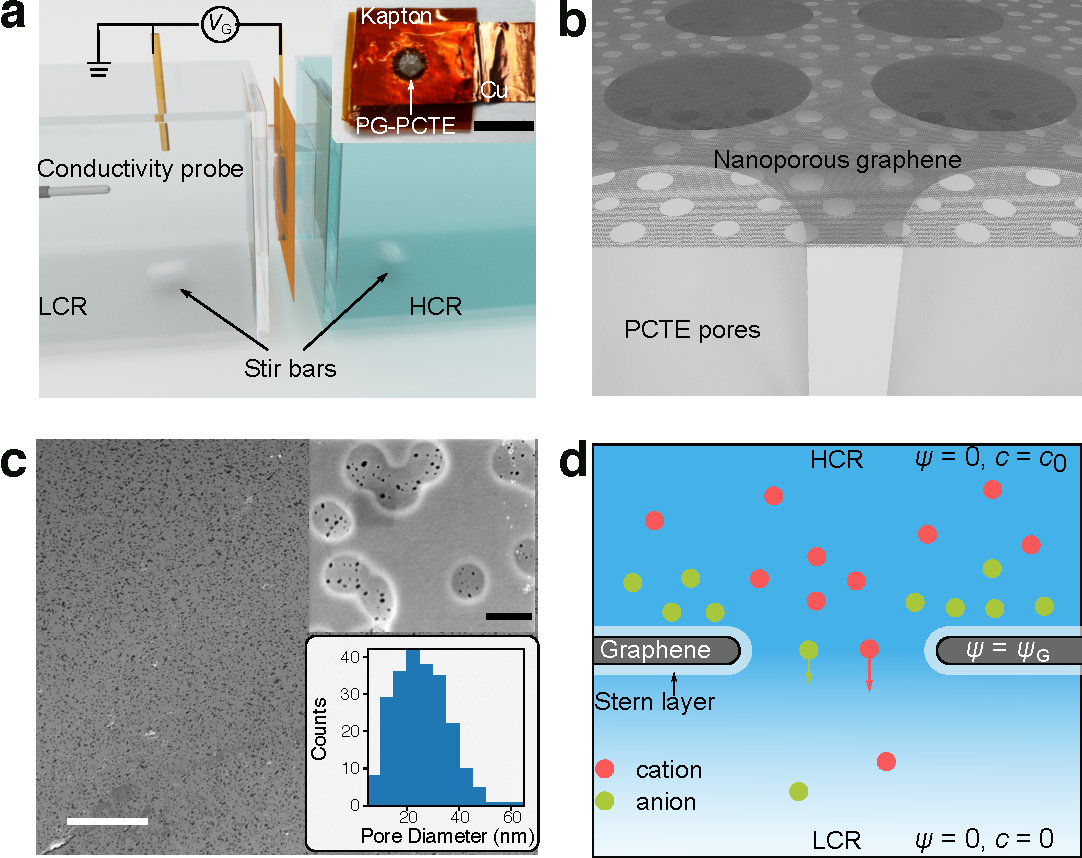
\includegraphics[width=0.95\linewidth]{img/fig1.pdf}
  \caption{\textbf{Experimental setup and nanopore characterization}.
    \textbf{a}. 3D schematic diagram showing the experimental
    setup. Inset: photograph of the PG-PCTE membrane supported by
    Kapton and copper tapes. (Scale bar: 1 cm.) \textbf{b}. 3D schematic
    of the nanoscale cross-sectional structure of the PG-PCTE
    membrane. \textbf{c}. SEM image of the PG-PCTE membrane, showing an
    excellent coverage of graphene over the PCTE substrate, scale bar:
    20 $\mathrm{\mu}$m.  Upper right inset: high-resolution SEM image
    of individual nanopores on PG fabricated by the patterning
    technique. (Scale bar: 500 nm.) Bottom right inset: histogram of the
    pore diameter distribution revealed by the SEM
    image. \textbf{d}. Schematic of the nanoscale ionic transport
    through a gated graphene nanopore.}
  \label{fig:1}
\end{figure}

\begin{figure}[htbp]
  \centering
  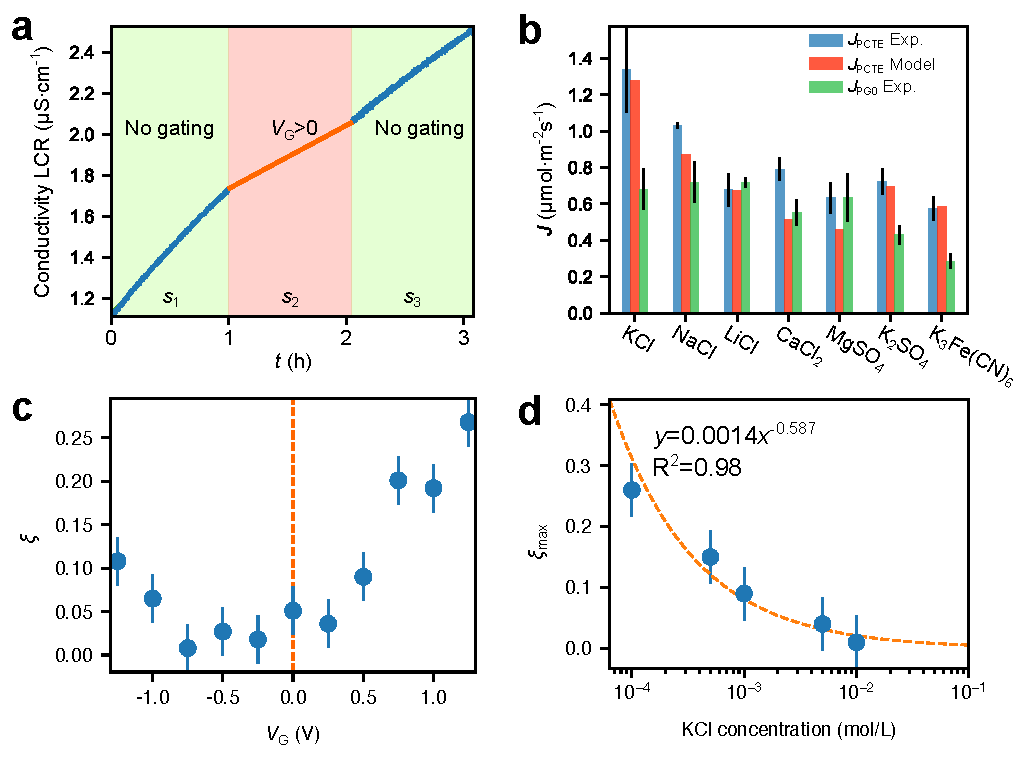
\includegraphics[width=0.95\linewidth]{img/fig2.pdf}
  \caption{\textbf{The experimental evidence of salt rejection.}
    \textbf{a}.An example of measured conductivity in LCR as a
    function of time. The slope of conductivity-time curve when
    $V_{\mathrm{G}}>0$ is interpolated, is smaller than that without
    gating. \textbf{b}. Molar diffusive flux through bare PCTE (blue
    bars: experimental; red bars: model values) and PG+PCTE (green
    bars) membranes for different salts. \textbf{c}. Experimentally
    measured salt rejection factor $\xi$ as a function of
    $V_{\mathrm{G}}$ for 0.1 mM KCl solution in HCR, showing an
    asymmetric response, with a higher degree of salt rejection for
    $V_{\mathrm{G}}>0$. \textbf{d}. $\xi_{\mathrm{max}}$ as a function
    of KCl concentration, fitted by a power law relation, suggesting
    the effect of Debye length on the observed salt rejection, since
    $\lambda_{\mathrm{D}} \propto c_{0}^{-\frac{1}{2}}$.}
  \label{fig:2} 
\end{figure}

\begin{figure}[htbp]
  \centering
  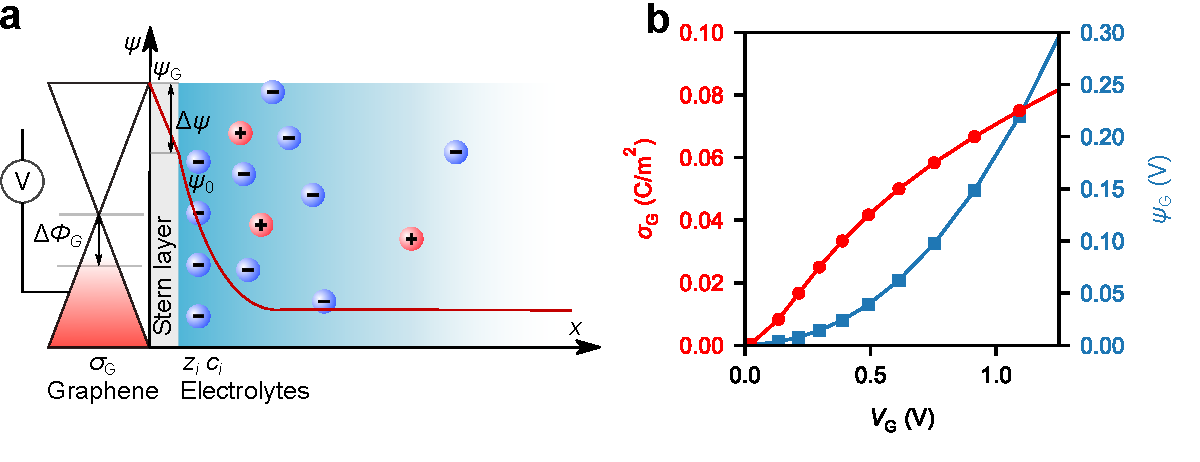
\includegraphics[width=0.95\linewidth]{img/fig3.pdf}
  \caption{\textbf{Interplay between graphene quantum capacitance and
      EDL.} \textbf{a}. Schematic diagram of the electric
    potential at the graphene-electrolyte interface considering the
    quantum capacitance of graphene. The interfacial potential of the
    electrolyte solution, $\psi_{0}$, is smaller than the bias
    $V_{\mathrm{G}}$ applied, as a result of the change of graphene's
    Fermi level $\Delta \phi_{\mathrm{G}}$ and the potential drop in
    the Stern layer $\Delta \psi$. \textbf{b}. Calculated surface
    charge $\sigma_{\mathrm{G}}$ and surface potential
    $\psi_{\mathrm{G}}$ of graphene as a function of $V_{\mathrm{G}}$
    in a 1 mM KCl solution. }
  \label{fig:3}
\end{figure}

\begin{figure}[htbp]
  \centering
  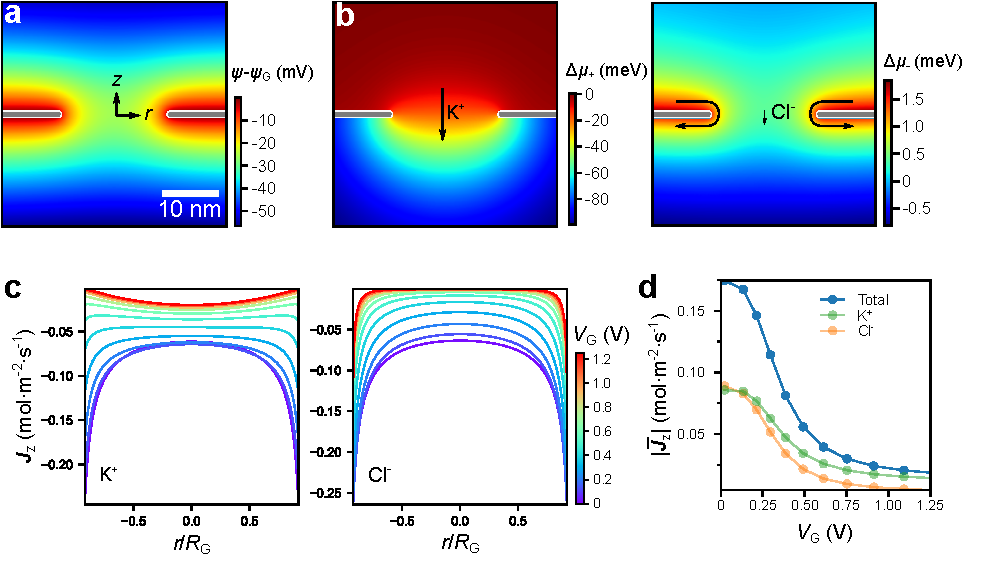
\includegraphics[width=0.95\linewidth]{img/fig4.pdf}
  \caption{\textbf{Calculations using the proposed self-consistent
      theory}. \textbf{a}. Calculated cross-sectional contour plot of
    electric potential $\psi$ near the center of the graphene
    nanopore at $V_{\mathrm{G}}$ = 0.75 V. \textbf{b}. The
    corresponding electrochemical potential change for cation
    $\Delta \mu_{+}$ (left) and anion $\Delta \mu_{-}$ (right). The
    reference of electrochemical potential is set in the HCR far from
    the graphene layer. The diffusive pathways for both ions are
    indicated by the arrows. \textbf{c}. Calculated z-component of
    diffusive fluxes $\boldsymbol{J}_{z}$ for cation (left) and anion
    (right) through the pore as functions of the relative position
    inside the pore, considering different levels of $V_{\mathrm{G}}$
    applied. \textbf{d}. Calculated z-components of cation, anion, and
    total fluxes through the graphene nanopore as functions of
    $V_{\mathrm{G}}$, showing salt rejection for all fluxes.}
  \label{fig:4}
\end{figure}

\begin{figure}[htbp]
  \centering
  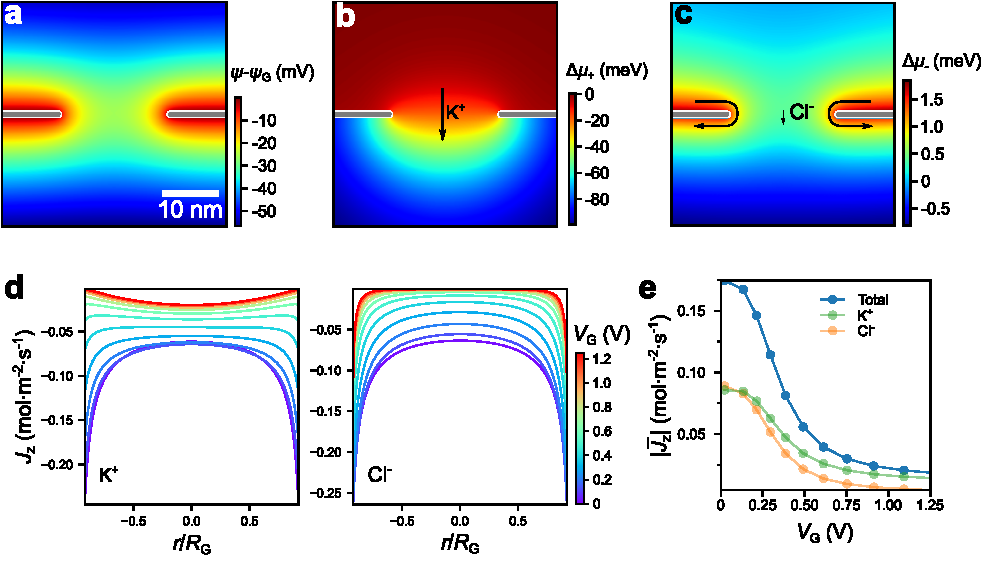
\includegraphics[width=0.95\linewidth]{img/fig5.pdf}
  \caption{\textbf{The Debye length effect on the degree of salt
      rejection}. \textbf{a}. Calculated contour plot of the surface
    potential of graphene $\psi_{\mathrm{G}}$ as a function of
    $\lambda_{\mathrm{D}}/r_{\mathrm{G}}$ and $V_{\mathrm{G}}$. When
    the Debye length reduces, a higher $V_{\mathrm{G}}$ is required to
    maintain the same surface $\psi_{\mathrm{G}}$
    level. \textbf{b}. Calculated 2D contour plot of theoretically
    predicted $\xi$ as a function of
    $\lambda_{\mathrm{D}}/r_{\mathrm{G}}$ and
    $V_{\mathrm{G}}$. Clearly, a higher degree of salt rejection can
    be achieved by having a higher $V_{\mathrm{G}}$ and
    $\lambda_{\mathrm{D}}/r_{\mathrm{G}}$}
  \label{fig:5}
\end{figure}

\begin{figure}[htbp]
  \centering
  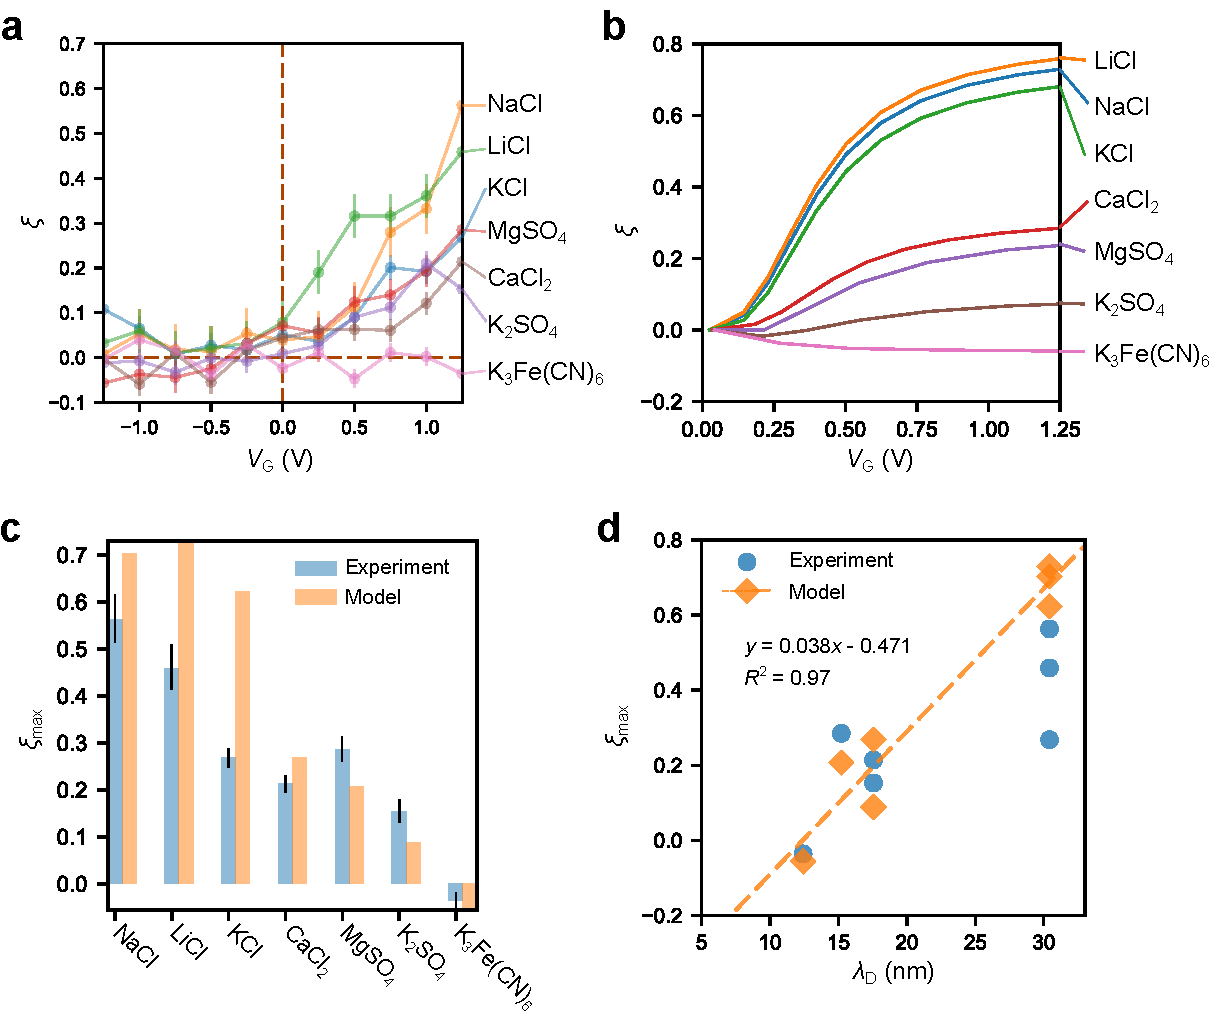
\includegraphics[width=0.95\linewidth]{img/fig6.pdf}
  \caption{\textbf{Comparison between experimental and theoretical
      salt rejection considering different salt
      species}. \textbf{a}. Experimentally measured $\xi$ as a
    function of $V_{\mathrm{G}}$ for various salts at 0.1 mM. The
    error bar represents the standard error. \textbf{b}. Theoretically
    calculated $\xi-V_{\mathrm{G}}$ relations for the salt species
    considered here. \textbf{c}. Comparison between the experimental
    and calculated $\xi_{\mathrm{max}}$ values for different salt
    species, decreasing with the salt
    valence. \textbf{d}. $\xi_{\mathrm{max}}$ as a function of
    $\lambda_{\mathrm{D}}$ for the experimental (circle) and model
    (diamonds) values, showing a linear correlation.}
  \label{fig:6}
\end{figure}

%%%%%%
%%Begin SI part
%%%%%%



\clearpage{}
\includepdf[page=-]{SI_titlepage.pdf}
\clearpage{}

\setcounter{page}{1}
\setcounter{section}{0}
\setcounter{equation}{0}
\setcounter{figure}{0}
\setcounter{table}{0}
\renewcommand{\thepage}{S\arabic{page}}
\renewcommand{\thesection}{S\arabic{section}}
\renewcommand{\theequation}{S\arabic{equation}}
\renewcommand{\thefigure}{S\arabic{figure}}
\renewcommand{\thetable}{S\arabic{table}}


\section{Graphene membrane manufacturing and results.}
\label{sec:exp}

\begin{figure}[htbp]
  \centering
  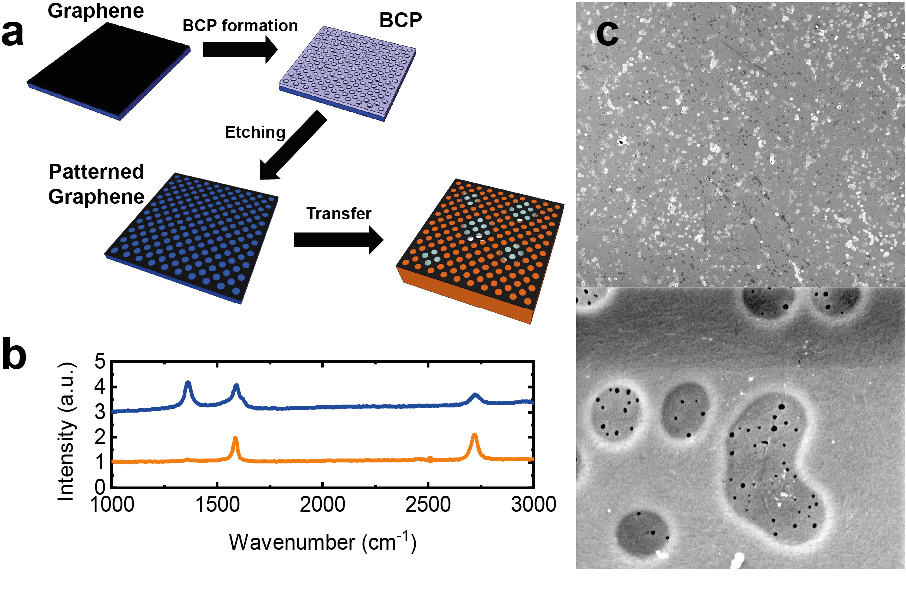
\includegraphics[width=0.95\linewidth]{img/SI-1.png}
  \caption{Fabrication and characterization of porous graphene membranes. \textbf{a}. Schematic of manufacturing process for
    patterning of double layer graphene. Graphene is synthesized and
    transferred to a substrate (glass slide) to yield a double
    layer. s-BCP is spin-coated and annealed in vacuum to undergo microphase
    separation, followed by plasma etch and wet etching yielding a
    porous polystyrene (PS) mask. Anisotropic etching of the mask
    leads to patterning the underlying graphene, PS is removed by
    thermal annealing. The porous graphene is then transferred to a
    substrate (e.g. PCTE). \textbf{b}. Raman spectra of graphene
    before (orange curve) and after (blue
    curve) patterning. An increase of the D-peak at 1350 cm$^{-1}$ indicates the
    formation of defects and edges. The spectra have been normalized
    to the G-peak intensity and offset for better
    comparison. \textbf{c}. SEM graph of patterned graphene on PCTE at
    lower (top) and higher (bottom) magnifications.
    % Note that tears in
    % graphene appear bright white with a black center.
  }
  \label{fig:exp}
\end{figure}

\section{Ion diffusion measurement and calculation}
\label{sec:measure}

The ion diffusion through b-PCTE has been performed using a sample
sandwiched between two layers of Aluminum tape where the edges have
been sealed using water-resistant epoxy (ACS Marine Epoxy) to avoid
interlayer leakage pathways \cite{Choi_2018}.  The sample was inserted in
the fixture following the same wetting procedure described in the main
text Methods and was kept wet for the entire series of experiments.

\begin{table}[htbp]
  \centering
  \begin{tabular}{lc}
    \hline
    Salt & $D$ (10$^{-9}$ m$^{2}\cdot$s$^{-1}$) \\
    \hline
    K$^{+}$     & 1.95 \\
    Na$^{+}$    & 1.33 \\
    Li$^{+}$    & 1.03 \\
    SO$_{4}^{2-}$       & 1.06 \\
    Ca$^{2+}$   & 0.79\\
    Mg$^{2+}$ & 0.7\\
    Fe{[(CN)$_{6}$]}$^{3-}$   & 0.90\\
    Cl$^{-}$ &  2.03 \\
               \hline
  \end{tabular}
  \caption{Different diffusivity values for the anions and cations of the
    salts used in this work \cite{vanysek_2000}. The theoretical
    diffusion through PCTE can be calculated using Eq. 1 in the main
    text and the diffusivities of the respective anion and cation.}
  \label{tab:diff}
\end{table}

The conductivity increase $s$ (mS$\cdot$cm$^{-1}\cdot$d$^{-1}$) is
converted into ion permeation rates $\boldsymbol{J}_{\mathrm{PCTE}}$
(mol$\cdot$m$^{-2}\cdot$s$^{-1}$) by use of a calibration factor
$c_{\mathrm{f}}$, the volume of LCR ($V_{\mathrm{LCR}}$) , the area of
the membrane $A$ and the time $t$ as:
\begin{equation}
  \label{eq:JPCTE}
  \boldsymbol{J}_{\mathrm{PCTE}} = \frac{s V_{\mathrm{LCR}}}{c_{\mathrm{f}} A t}
\end{equation}
The calibration factors for all salts have been obtained by a linear
fit of conductivity \textit{versus} concentration for 4 solutions with
concentrations from 10$^{-4}$ M to 10$^{-2}$ M and extracting the
resulting slope. The rest of the factors are $V_{\mathrm{LCR}}$ = 7.33
mL, $A$ = 9$\times$10$^{-6}$ m$^{2}$. Table \ref{tab:exp-2} shows the
averaged conductivity increase s, the extracted calibration factors
$c_{\mathrm{f}}$ and the resulting ion permeation rates using
Eq. \ref{eq:JPCTE}. The values from this table are shown in main text \Fig 2b
(blue bars).
\begin{table}[htbp]
  \centering
  \begin{tabular}{lccc}
    \hline
    Salt & $s$ (mS$\cdot$cm$^{-1}$d$^{-1}$) & $c_{\mathrm{f}}$ (mS$\cdot$cm$^{-1}\cdot$mol$^{-1}\cdot$L) &
                                                                                                            $\boldsymbol{J}_{\mathrm{PCTE}}$ (10$^{6}$ mol$\cdot$m$^{-2}\cdot$s$^{-1}$)\\
    \hline
    KCl & 1.51$\pm$0.27$\times$10$^{-2}$  & 106   & 1.34 $\pm$ 0.24\\
    NaCl        & 9.90$\pm$0.17$\times$10$^{-3}$ & 91    & 1.02 $\pm$ 0.02\\
    LiCl        & 6.03 $\pm$0.80$\times$10$^{-3}$        & 83    & 0.682 $\pm$ 0.090\\
    CaCl$_{2}$  & 1.25$\pm$0.1$\times$10$^{-2}$    & 149   & 0.789 $\pm$ 0.063\\
    MgSO$_{4}$  & 8.80$\pm$1.2$\times$10$^{-3}$   & 130   & 0.633 $\pm$ 0.084\\
    K$_{3}$[Fe(CN)$_{6}]$ & 2.40$\pm$0.28$\times$10$^{-2}$   & 395   & 0.575 $\pm$ 0.063\\
    K$_{2}$SO4$_{4}$    & 1.98$\pm$0.20$\times$10$^{-2}$  & 258   & 0.722 $\pm$ 0.073\\
    \hline
  \end{tabular}
  \caption{Extracted slope $s$ as an averaged result from 3 consecutive
    measurements, the calibration factors $c_{\mathrm{f}}$ and the resulting ion
    permeation $\boldsymbol{J}_{\mathrm{PCTE}}$ through b-PCTE membranes for all salts.}
  \label{tab:exp-2}
\end{table}

The experimentally observed flux reduction through PG-PCTE upon
gating, $\eta$, for all the salts studied here (with concentration of
0.1 mM in HCR), can be found in Fig. \ref{fig:eta-all}. The effective salt
rejection ratio $\xi$ is then extracted using main text
Eq. \ref{eq:xi-def}.

\begin{figure}[htbp]
  \centering
  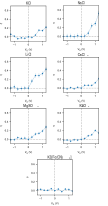
\includegraphics[width=0.5\linewidth]{img/SI-eta-all.pdf}
  \caption{Measured $\eta$ values as function of $V_{\mathrm{G}}$ for
    various salts used in this work. The concentration in HCR is 0.1
    mM in all cases.}
  \label{fig:eta-all}
\end{figure}


\section{Control experiment with copper tape}
\label{sec:copper}
We make sure that the applied voltage is effectively applied via the
graphene membrane and not through leakage directly coupling the
copper tape to the ionic solution. For this purpose, we use a device as in \Fig
1a, omitting the graphene and measuring the current through the
membrane with the Autolab electrochemical workstation using the
membrane as working electrode and a platinum wire as counter/reference
electrode 3.5 cm apart in 0.1 mM KCl. When no graphene is inserted in
the device, a current in the baseline range ($\sim$ 0.1 nA) is
observed, indicating no current passing from the membrane. However, if
graphene is inserted, a current in the range of $\sim$ 10 - 100 nA is
measured. If the copper tape is in contact with the solution when
omitting the Kapton tape, the current increases to $\sim$ 1 - 10
$\mathrm{\mu}$A, independent of the exposed area of the copper tape to
the solution.

% \pagebreak

\section{Circuit analog model of transport through PG-PCTE}
\label{sec:R-model}

\begin{figure}[htbp]
  \centering
  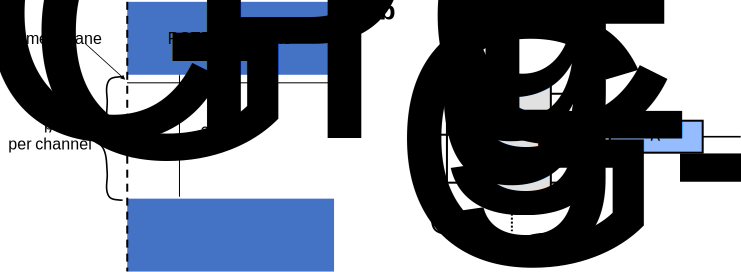
\includegraphics[width=0.8\linewidth]{img/SI-resistance-rejection.pdf}
  \caption{Simple circuit analog model for the transport through
    PG-PCTE membrane. \textbf{a}. Schematic of PG-PCTE membrane in
    cross-section view. \textbf{b}. Model for transport resistance in
    analogy to an electric circuit. This schematic depicts a cut
    through a PG-PCTE membrane showing a single PCTE pore and multiple
    graphene pores.}
  \label{fig:R-model}
\end{figure}
The ionic transport through the PG-PCTE membrane is the concerted
effect the transport resistance through PG and PCTE membranes,
respectively. As schematically shown in Fig. \ref{fig:R-model}, the
overall transport resistance of the system is composed of the series
resistance $R_{\mathrm{G}}$ and $R_{\mathrm{PCTE}}$, respectively. For
both PG and PCTE membranes, the resistance $R$ is defined as the ratio
between the concentration between HCR and LCR $\Delta c$, and the total diffusive current $I$ as:
\begin{equation}
\label{eq:1}
R_{i} = \Bigg|\frac{\Delta c}{I_{i}}\Bigg| =  \Bigg|\frac{\Delta c}{J_{i}A_{i}}\Bigg|
\end{equation}
where $i$ denotes the membrane type and $A_{i}$ is the area of the
pore. We further treat $R_{\mathrm{G}}$ as the effective resistance of
$\gamma$ parallel resistors with individual resistance
$R_{\mathrm{g}}$, where $\gamma$ is the average number of PG pores per
PCTE channel, and $R_{\mathrm{g}}$ is the average transport resistance
per PG pore. The value of $\gamma$ is determined from geometric
analysis of both membranes: given the pore number density of PG
($\sim$1.25$\times$10$^{14}$ m$^{-2}$), the pore number density of
PCTE ($\sim$1.50$\times$10$^{12}$ m$^{-2}$), and the percentage of
PCTE pores with PG on top ($\sim$0.13), $\gamma$ is determined to be
$\sim$10.83.

The objective of the circuit analog model is to find effective salt
rejection ratio through PG, $\xi$ extracted from the experimental
$\eta$ values (defined in main text Eq. \ref{eq:rejection}). By
defining $R_{\mathrm{G}}^{0}=R_{\mathrm{G}}(V_{\mathrm{G}}=0)$,
$\delta = R_{\mathrm{PCTE}} / R_{\mathrm{G}}^{0}$,
$\chi = R_{\mathrm{G}}/R_{\mathrm{G}}^{0}$, $\eta$ is rewritten using
transport resistances as:
\begin{equation}
  \begin{aligned}[t]
      \label{eq:eta-R}
  \eta &= 1 - {\displaystyle
    \left[\frac{(R_{\mathrm{PCTE}} + R_{\mathrm{G}})}
    {(R_{\mathrm{PCTE}} + R_{\mathrm{G}}^{0})}\right]^{-1}} \\
    &= 1 - \frac{\delta + 1}{\delta + R_{\mathrm{G}}/R_{\mathrm{G}}^{0}} \\
    &= 1 - \frac{\delta + 1}{\delta + \chi}
  \end{aligned}
\end{equation}
Consequentially, the
salt rejection ratio $\xi$, is associated with $\chi$ by
$\xi = 1 - \chi^{-1}$ and is related with $\delta$ and $\eta$ via:
\begin{equation}
  \label{eq:xi-deriv}
  \begin{aligned}[t]
    \xi &= 1 - \chi^{-1} \\
    &= \frac{(\delta + 1) \eta}{\delta\eta + 1}
  \end{aligned}
\end{equation}
which is main text Eq. \ref{eq:xi-def}. When $0<\eta<1$ (salt
rejection regime) and $\delta>0$, Eq. \ref{eq:xi-deriv} always
guarantees $\xi>\eta$, since $\delta + 1$ is always larger than
$\delta\eta + 1$. In other words, due to the existence of
$R_{\mathrm{PCTE}}$, the effective salt rejection through PG upon
gating is always larger than that experimentally observed.

Next we seek the value of $\delta$, the resistance ratio
between the PCTE and PG membranes, without gating. The range
of $\delta$ can be estimated from experimental data in main text
Fig. \ref{fig:2}b using the relation:
\begin{equation}
  \label{eq:exp-delta}
  \delta = \left(\frac{\boldsymbol{J}_{\mathrm{PCTE}}}{\boldsymbol{J}_{\mathrm{PG}}^{0}} -1 \right)^{-1}
\end{equation}
by assuming the validity of the circuit analog model for all salt
systems. As shown in Fig. \ref{fig:delta-compare}, the
experimentally estimated value of $\delta$ varies from 1 to 5,
indicating that the resistance of the PG membrane is dominating in the
PG-PCTE system.
\begin{figure}[htbp]
  \centering
  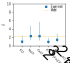
\includegraphics[width=0.55\linewidth]{img/SI-delta-estimate.pdf}
  \caption{Comparison between the $\delta$ value estimated from simple
    geometric model (Eq. \ref{eq:delta-resistance}) and from
    experimental value (Eq. \ref{eq:exp-delta}), showing good
    agreement between the two methods.  }
  \label{fig:delta-compare}
\end{figure}
$\delta$ can also be estimated using geometric parameters of both
membranes. For a long PCTE channel with length $L$ and
$r_{\mathrm{PCTE}}$, $R_{\mathrm{PCTE}}$ has power law of
$L/r_{\mathrm{PCTE}}^{2}$, while for a graphene pore
with radius $r_{\mathrm{G}}$ and vanishing thickness, the resistance of individual pore $R_{\mathrm{g}}^{0}$
has power law $1/r_{\mathrm{G}}$ \cite{O_Hern_2014}, which are expressed as:
\begin{subequations}
\begin{eqnarray}
  \label{eq:R-both}
  R_{\mathrm{PCTE}} &= &k_{\mathrm{PCTE}} \frac{L}{r_{\mathrm{PCTE}}^{2}} \\
  R_{\mathrm{g}}^{0} &= &k_{\mathrm{g}} \frac{1}{r_{\mathrm{G}}}
\end{eqnarray}
\end{subequations}
where $k_{\mathrm{PCTE}}$ and $k_{\mathrm{g}}$ are the coefficient
associated with PCTE and PG membranes, respectively. The value of
$\delta$ is then expressed as:
\begin{equation}
  \label{eq:delta-resistance}
  \delta
  = \frac{R_{\mathrm{PCTE}}}{R_{\mathrm{G}}^{0}}
  = {\displaystyle
    \frac{k_{\mathrm{PCTE}}}{k_{\mathrm{g}}}
    \frac{L r_{\mathrm{G}} \gamma}
        {r_{\mathrm{PCTE}}^{2}}}
\end{equation}
Here we take $L$=24 $\mu$m, $r_{\mathrm{G}}$=10 nm,
$r_{\mathrm{PCTE}}$=200 nm. From simple Fick's law,
the coefficient $k_{\mathrm{PCTE}}$ is determined as
$1/(D_{\mathrm{\pm}} \pi)$. On the other hand $k_{\mathrm{G}}$ varies
by the choice of model, ranging from $3 \pi / D_{\mathrm{\pm}}$ using
the analog of the Sampson formula for
fluid\cite{Roscoe_1949,Celebi_2014}, to $1/(2 D_{\mathrm{\pm}})$ from
the Hill formula for disk absorption model
\cite{Hill_1975,Grebenkov_2018}. As a result the theoretical value of
$\delta$ has lower bound of $\sim$2.2 (Sampson formula, orange line in
Fig. \ref{fig:delta-compare}) to $\sim$40.5 (Hill formula). We note
our experimental values of $\delta$ is in good agreement estimated
from the Sampson formula (which we use in the main text) while lower
than the Hill formula. Having a higher estimated value of $\delta$
could yield unreasonably high value of $\xi$ and the influence of
concentration is deviated from our theoretical predictions. Further
theoretical analysis taking nonidealities including surface adsorption
and chemical nature of pore edge, is required to have better
understanding of graphene's transport resistance.


% On the other hand, the transport through
% 2D pore with high radius/thickness ratio falls into the regime of the
% Sampson formula \cite{Roscoe_1949}, where the entrance resistance
% dominates over the bulk resistance, with the formula as
% \cite{Roscoe_1949,Celebi_2014}:
% \begin{equation}
%   \label{eq:sampson}
%   R_{\mathrm{g}}^{0} = \frac{1}{D} \frac{3 \pi}{r_{\mathrm{G}}}
% \end{equation}
% We therefore estimate the value of $\delta$ as:




\section{KCl Debye length and conductivity}
\label{sec:debye}
Table \ref{tab:debye} gives an overview about the measured
conductivities and their calculated Debye length values for KCl. The
information is used to plot the $\xi$ versus $c_{0}$ curve.

\begin{table}[htbp]
  \centering
  \begin{tabular}{lccc}
    \hline
    $c_{0}$ (mM) & Conductivity (mS$\cdot$cm$^{-1}$) & $\lambda_{\mathrm{D}}$ (nm)\\
    \hline
    0.1&        1.90$\times$10$^{-2}$ &        30.4\\
    0.33&       5.41$\times$10$^{-2}$ & 16.0\\
    1   &1.33$\times$10$^{-1}$ & 10.0\\
    3.3&     5.13$\times$10$^{-1}$ &  6.0\\
    10&      1.08    &3.3\\
    \hline
  \end{tabular}
  \caption{Conductivity and calculated Debye lengths of various KCl
    concentrations in order to obtain rejection versus
    concentration curves. }
  \label{tab:debye}
\end{table}

\section{Measurement of charge carrier density of patterned graphene}
\label{sec:charge-dens}
The intrinsic charge carrier density of graphene was measured using a
field electron transistor (FET) in air with a 300nm SiO$_2$ as a
gate. The device setup is shown in Fig. \ref{fig:charge-dens}a,
where the source and drain electrodes were deposited onto the PG
sample transferred onto 300nm SiO$_2$ on doped Silicon. The
characteristic drain-source current $I_{\mathrm{DS}}$ as a function of
$V_{\mathrm{G}}$ is shown in Fig. \ref{fig:charge-dens}. The
charge-neutral point gate voltage $V_{\mathrm{CNP}}$ is measured to be 2.8 V.
Using the capacitance of the SiO$_{2}$ dielectric, we estimate an intrinsic
charge density of $\sim{}$1.4$\times$10$^{11}$
\textit{e}$\cdot$cm$^{-2}$, and a shift in the PG's Fermi level by
$\sim{}$48 meV, which is negligible compared with the gate-induced
charge density in our experiments. Therefore, the assumption that the
PG sample is intrinsic without gating, is justified.

\begin{figure}[htbp]
  \centering
  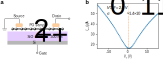
\includegraphics[width=0.8\linewidth]{img/SI-gr-transistor.pdf}
  \caption{Characterization of the intrinsic charge density of the PG
    sample using field effect transistor. \textbf{a}. The setup of the
    PG-FET. \textbf{b}. The I$_{\mathrm{DS}}$ as a function of
    $V_{\mathrm{G}}$. The charge neutral point gate voltage is
    determined as $\sim{}$2.8 V, corresponding to an intrinsic charge
    density of $\sim{}$1.4$\times$10$^{11}$
    \textit{e}$\cdot$cm$^{-2}$, which is negligible compared with the
    gate-induced charges.}
  \label{fig:charge-dens}
\end{figure}

\pagebreak

\section{Further discussion about the ionic pathway near the graphene pore}
\label{sec:conc}

In this section we provide a more detailed discussion about the
different ionic pathways through the graphene nanopore upon gating in
main text Fig. \ref{fig:4}b. As discussed in the main text, the
ionic migration arises from both diffusion (caused by
concentration gradient) and electrostatic drift (caused by electric
field).  The effect of salt rejection can be viewed as follows: when
$V_{\mathrm{G}}$ = 0, the flux $\boldsymbol{J}_{\mathrm{G}}$ is solely
contributed by the concentration gradient, while after applying a
positive $V_{\mathrm{G}}$, distinct pathways for cations /
anions are created and the drift flux counteracts the diffusion.

Applying a positive $V_{\mathrm{G}}$ changes the surface distribution
of the cations / anions. To see this, we plot the concentrations of
cations ($c_{+}$) and anions ($c_{-}$) near a graphene nanopore with
$r_{\mathrm{G}}$ = \unit[10]{nm}, $c_{0}$ = \unit[0.1]{mM} and $V_{\mathrm{G}}$ =
\unit[0.75]{V}, as shown in Fig. \ref{fig:conc}a and \ref{fig:conc}b,
respectively. The cations are depleted from the graphene surface,
while the anions are accumulated due to positive
$\psi_{\mathrm{G}}$. The anion concentration at the graphene surface
is enhanced $\sim{}$35 times compared with the bulk concentration in
HCR. The thickness of the depletion / accumulation layer is affected
by the bulk concentration. Here we show this by comparing the radial
distribution of $c_{+}$ and $c_{-}$ along the $z = 0$ line within the
graphene pore. Fig. \ref{fig:conc-r} shows such radial ionic
concentration distribution at different $c_{0}$ and $V_{\mathrm{G}}$
levels. When $c_{0}$ = \unit[0.1]{mM}, $\lambda_{\mathrm{D}}$ is larger than
$r_{\mathrm{G}}$, and the external gate voltage $V_{\mathrm{G}}$ has
control over both $c_{-}$ and $c_{+}$ within the graphene nanopore
(Fig. \ref{fig:conc-r}a and \ref{fig:conc-r}c). On the other
hand, when $c_{0}$ = \unit[100]{mM}, $\lambda_{\mathrm{D}}$ is much smaller
than $r_{\mathrm{G}}$, and the concentration is only affected by
$V_{\mathrm{G}}$ close to the pore edge (Fig. \ref{fig:conc-r}b
and \ref{fig:conc-r}d). Therefore by increasing $c_{0}$ (and
equivalently reducing $\lambda_{\mathrm{D}}$), $V_{\mathrm{G}}$ loses
control over the transport in the center of the pore and leads to a
lower $\xi$ value. Due to the existence of graphene's quantum
capacitance, the surface potential $\psi_{\mathrm{G}}$ is essentially
smaller than $V_{\mathrm{G}}$, and the maximum surface anion
concentration ($c_{0}$ = \unit[100]{mM}, $V_{\mathrm{G}}$ = \unit[1.25]{V}) is
$\sim{}$ \unit[3]{M}, much smaller than the saturated surface adsorption
density (at the order of \unit[10$^{2}$]{M}
\cite{bard_electrochemical_1980}). Therefore we expect the surface
enhancement of the anions under the FEM conditions to be realistic and
the influence of the anion concentration on the diffusivity is minimal
\cite{Tang_1999_I}.


\begin{figure}[htbp]
  \centering
  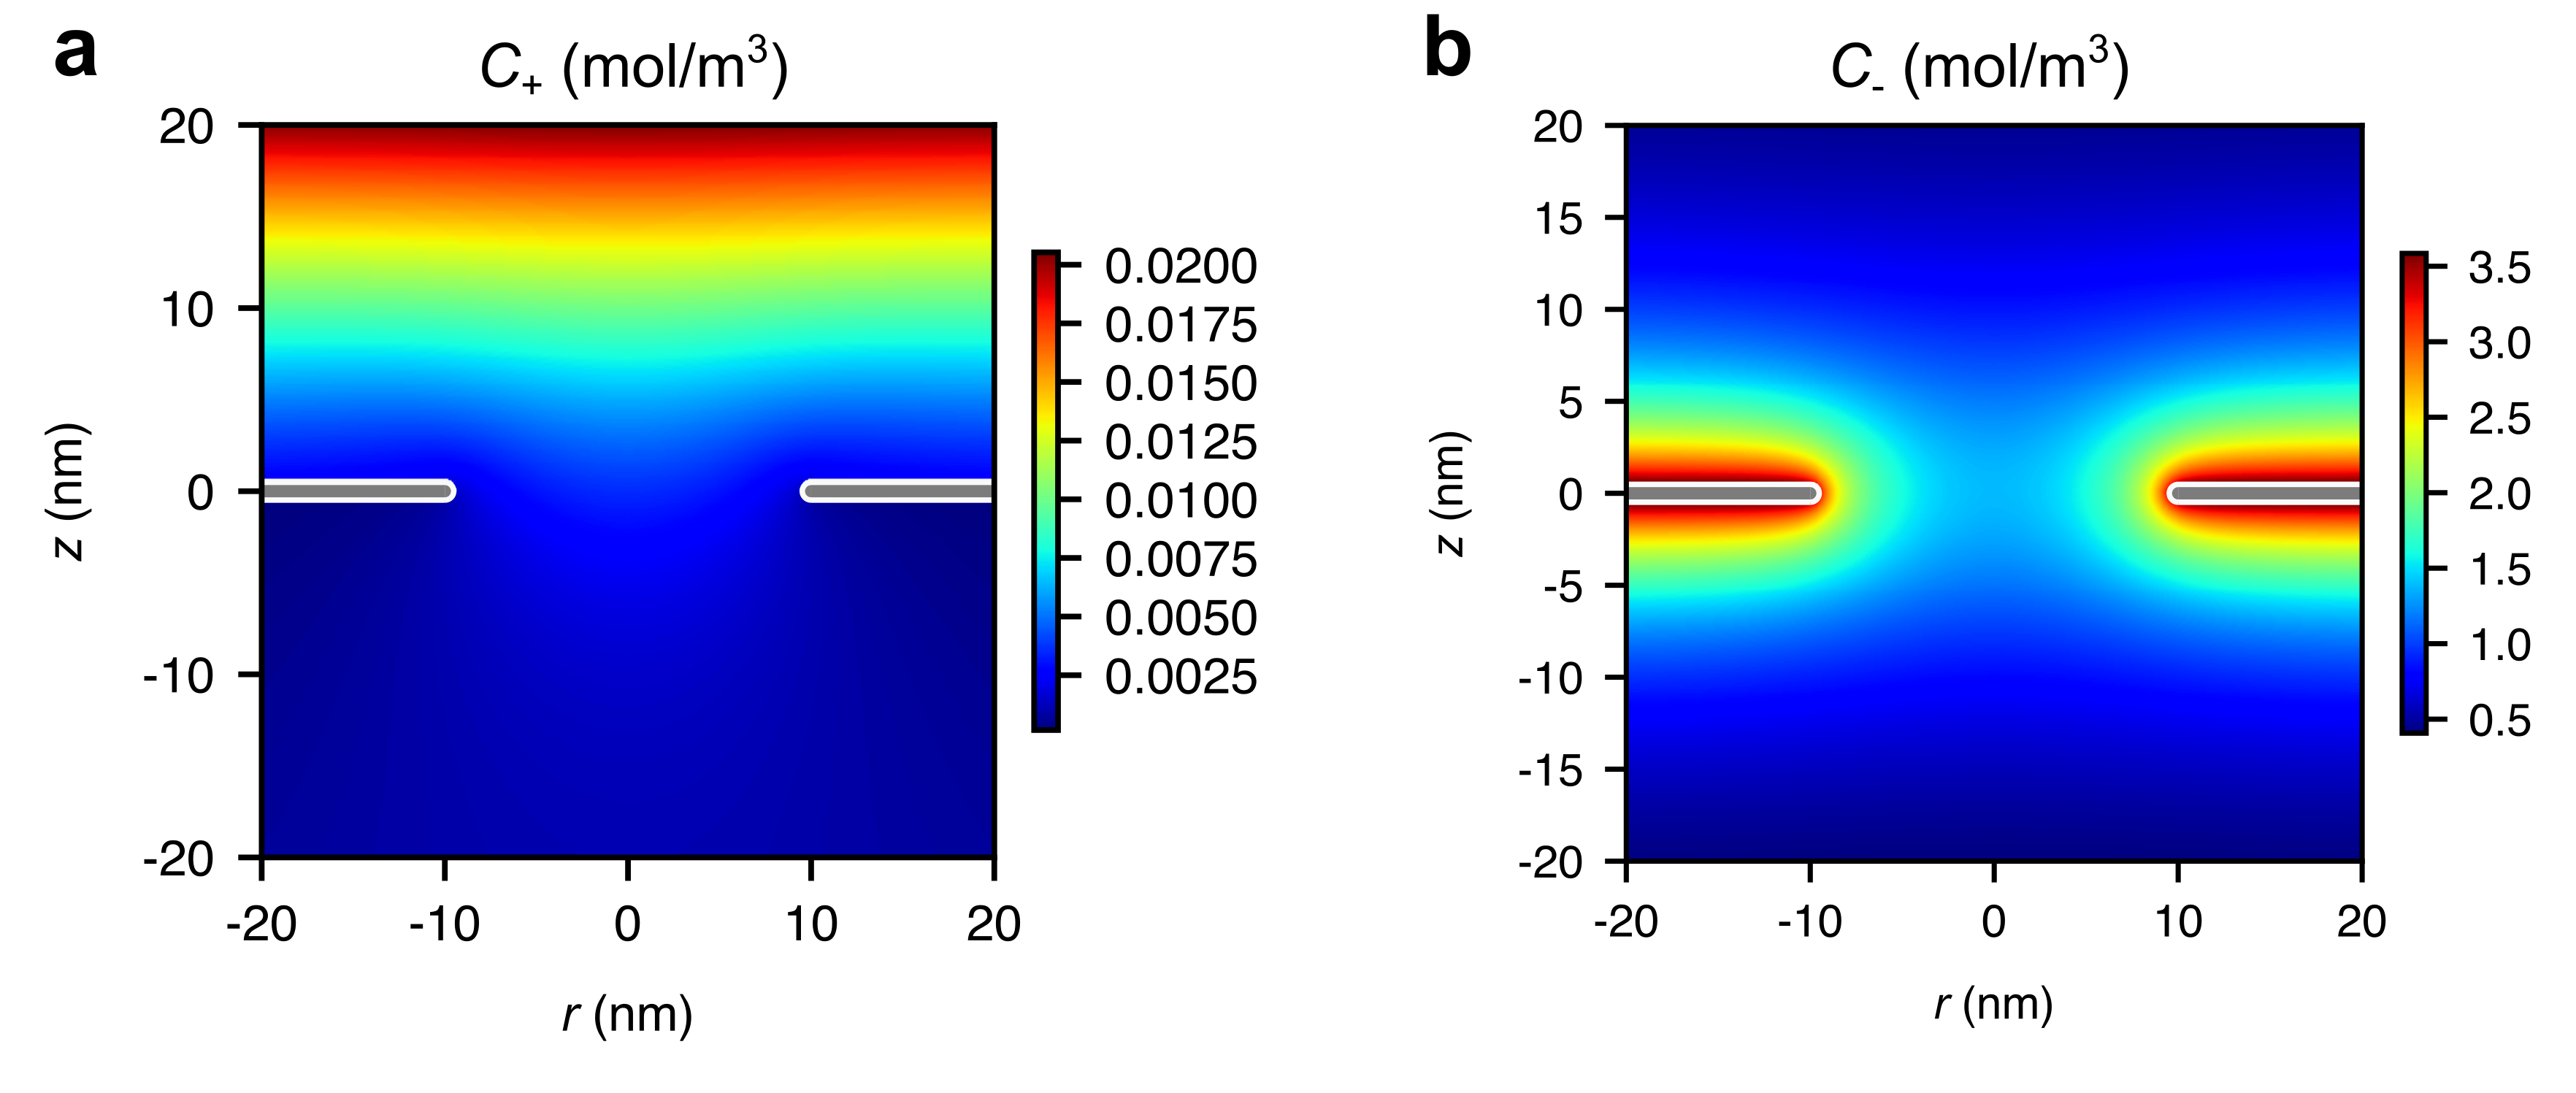
\includegraphics[width=0.8\linewidth]{img/SI-concentration.pdf}
  \caption{Cation concentration $c_{+}$ (\textbf{a}.) and anion
    concentration $c_{-}$ (\textbf{b}.) near the graphene nanopore
    with $r_{\mathrm{G}}$ = 10 nm, $c_{0}$ = 0.1 mM, and
    $V_{\mathrm{G}}$ = 0.75 V, for a KCl solution at 0.1
    mM. Depletion of cation and accumulation of anion can be observed
    near the graphene surface.}
  \label{fig:conc}
\end{figure}

\begin{figure}[htbp]
  \centering
  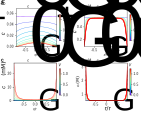
\includegraphics[width=0.75\linewidth]{img/SI-conc-r.pdf}
  \caption{Radial distribution of ions along the line $z=0$ within a
    graphene nanopore with $r_{\mathrm{G}}$ = 10 nm: (\textbf{a}.)
    $c_{+}$ at $c_{0}$ = 0.1 mM, (\textbf{b}.) $c_{+}$ at $c_{0}$ =
    100 mM, (\textbf{c}.) $c_{-}$ at $c_{0}$ = 0.1 mM and
    (\textbf{d}.) $c_{-}$ at $c_{0}$ = 100 mM. The lines with varied
    colors indicate the difference of $V_{\mathrm{G}}$ applied.}
  \label{fig:conc-r}
\end{figure}

Next we analyze the diffusion and drift contributions to the ionic
transport. As shown in Fig. \ref{fig:potential}, the
electrochemical potential energy $\mu_{i}$ is decomposed into the
electric potential energy $z_{i} c_{i} \psi_{i}$ (Fig.
\ref{fig:potential}a and \ref{fig:potential}b) and the chemical
potential energy $k_{\mathrm{B}}T \ln x_{i}$ (Fig.
\ref{fig:potential}c and \ref{fig:potential}d) near a graphene
nanopore with $r_{\mathrm{G}}$ = \unit[10]{nm} and $V_{\mathrm{G}}$ = \unit[0.75]
{V}. The transport of cations is dominated by its chemical potential and
the diffusion is most pronounced in the center of the pore. The electric and diffusive potentials are similar in magnitude, but with
opposite signs, counteracting each other. As a result, different pathways for cations
and anions emerge, where cations preferably pass through the pore
center, while anions mainly pass near the pore edge, as shown in
Fig. \ref{fig:flux}.

\begin{figure}[htbp]
  \centering
  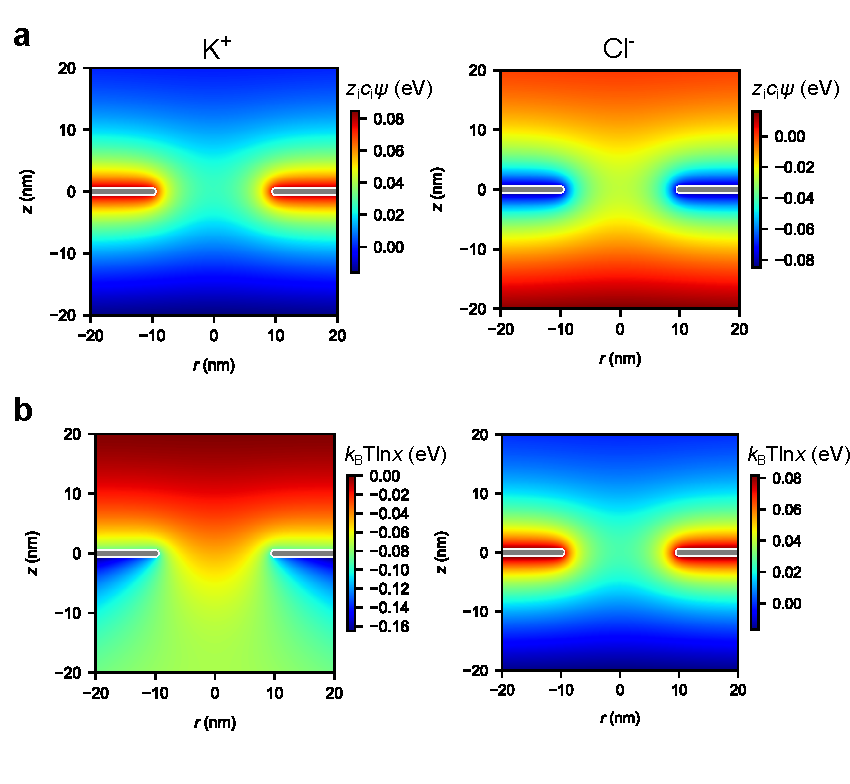
\includegraphics[width=0.8\linewidth]{img/SI-electrochemical-decomposite.pdf}
  \caption{Decomposition of electrochemical potential near a nanopore
    corresponding to main text \Fig \ref{fig:4}. \textbf{a}. The electrostatic
    (drift) contribution to the electrochemical potential for cation
    (left) and anion (right) and \textbf{b}. The concentration (diffusion)
    contribution to the electrochemical potential for cation (left)
    and anion (right). The relative small order of magnitude for anion
    electrochemical potential is caused by the balance between the
    diffusion and drift for anion.}
  \label{fig:potential}
\end{figure}

\begin{figure}[htbp]
  \centering
  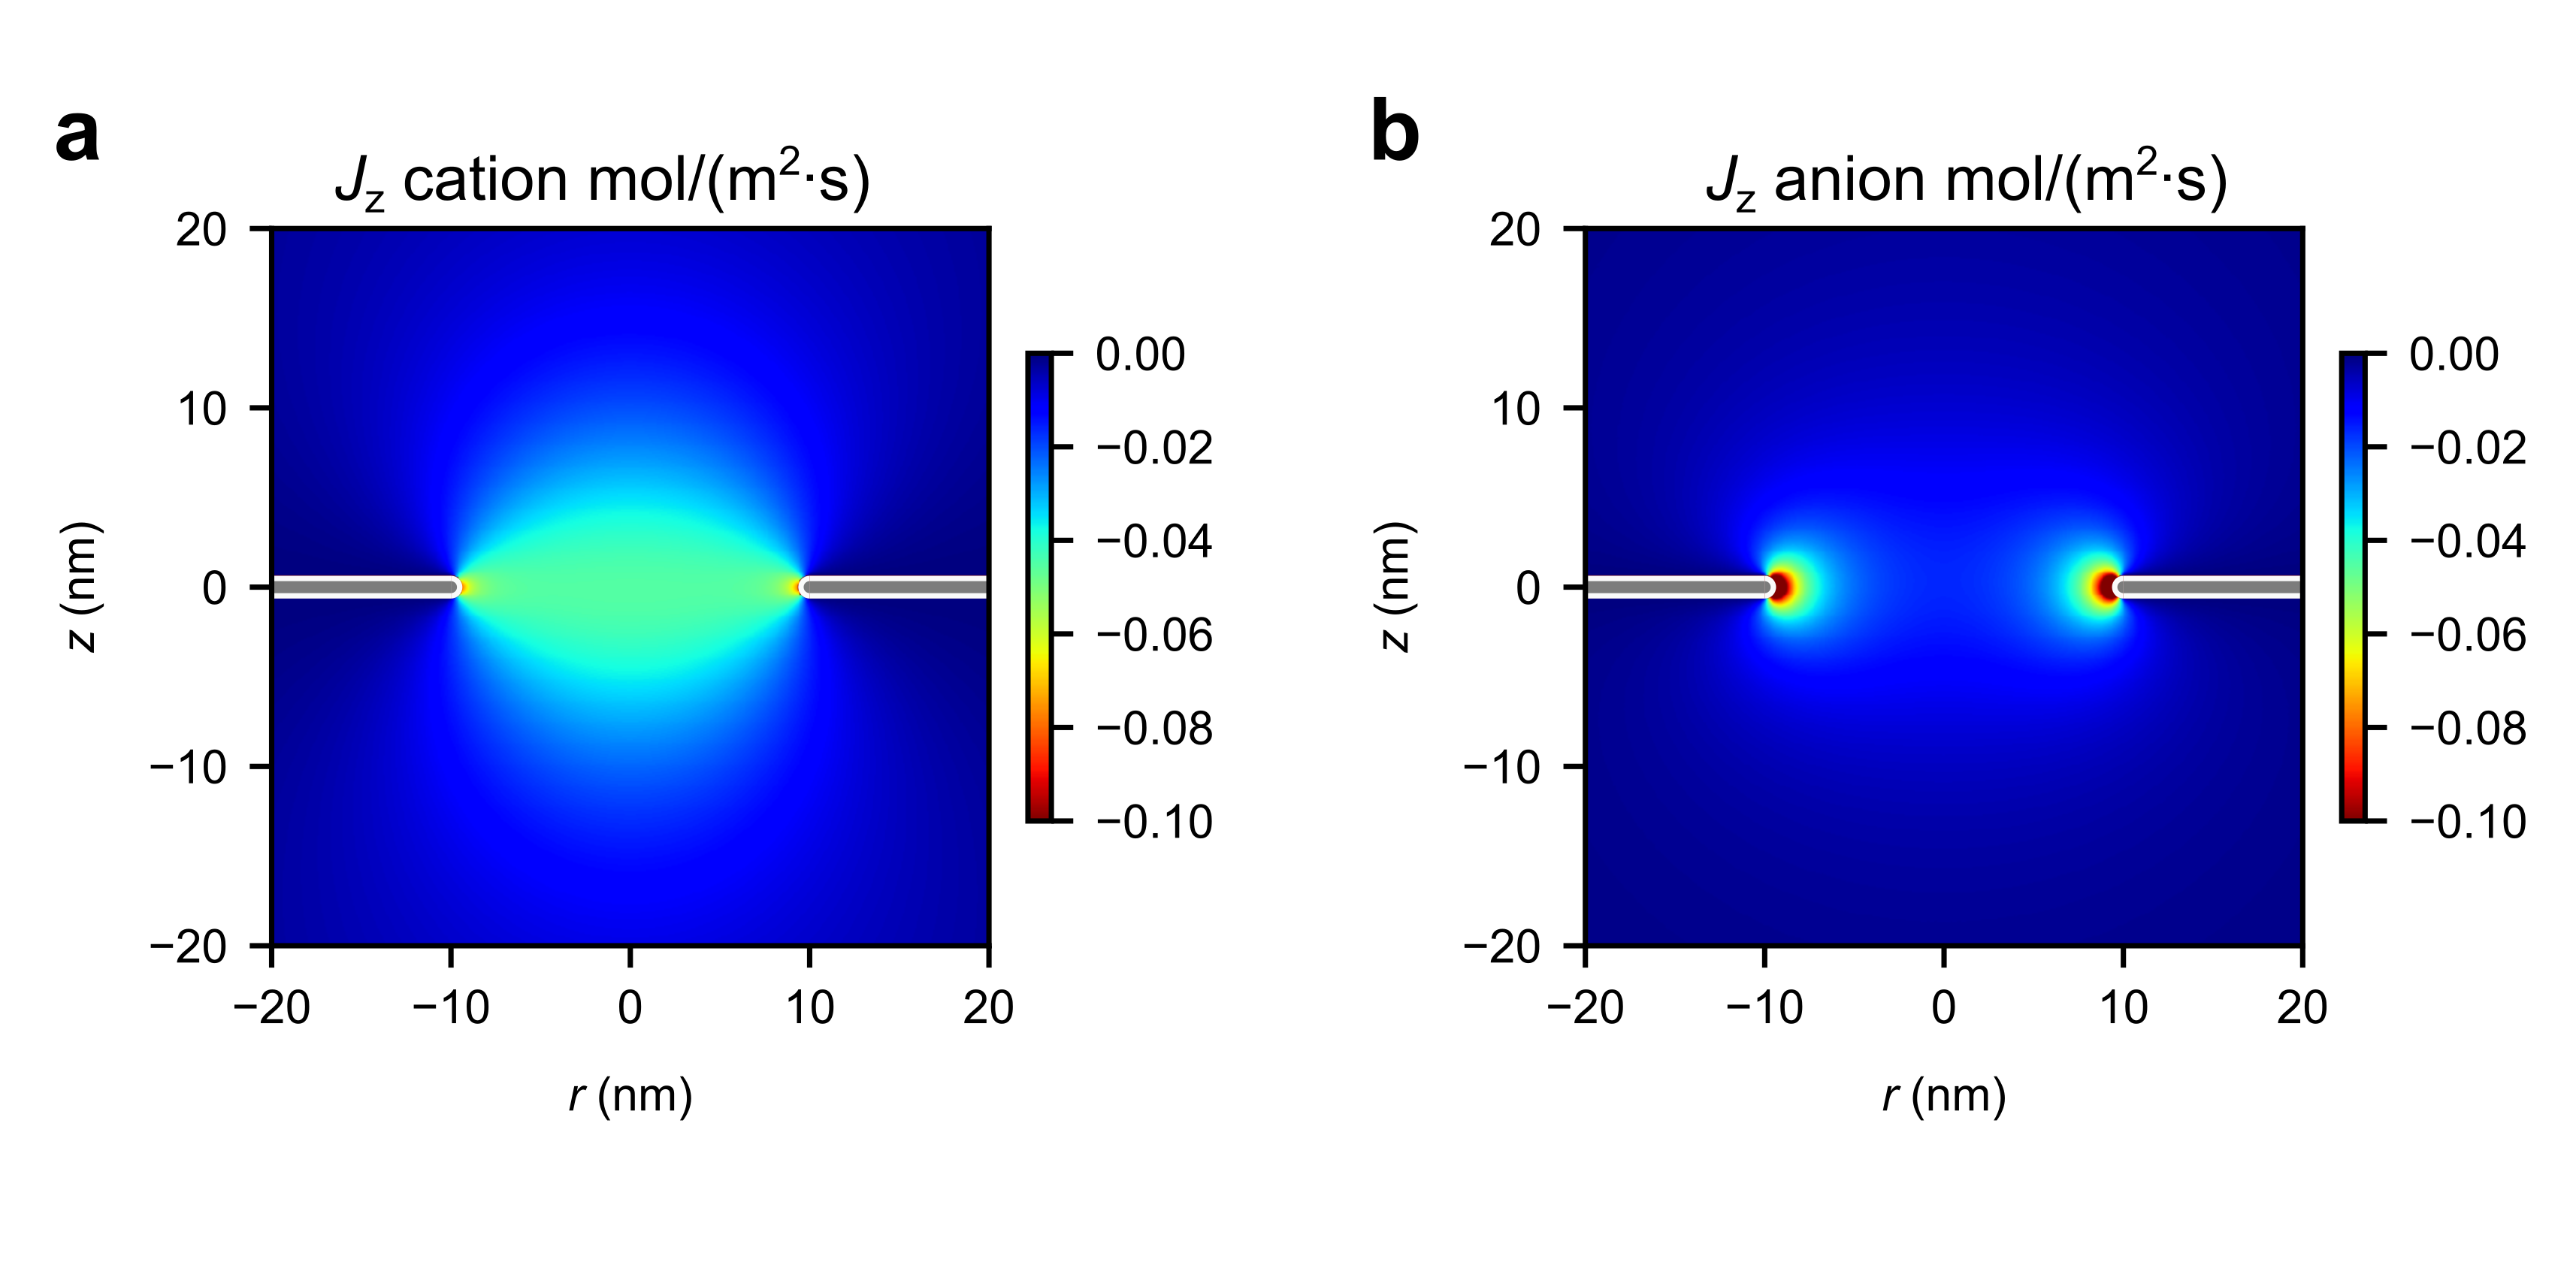
\includegraphics[width=0.8\linewidth]{img/SI-flux.pdf}
  \caption{z-component fluxes of cation ($J_{z+}$, \textbf{a}.)  and
    anion ($J_{z-}$ \textbf{b}.) near the graphene nanopore
    corresponding to Fig. \ref{fig:4}b in main text. The
    pathways for the different ions can be spatially distinguished:
    the flux of cation passes mostly through the center of the
    graphene nanopore while the anion passes mainly through the
    edge. The analysis is in consistent with the gradient of chemical
    potential as shown in the main text Fig. \ref{fig:4}b.}
  \label{fig:flux}
\end{figure}

We note that when the surface potential $\psi_{\mathrm{G}}$ of
graphene further increases, the salt rejection may be weakened, or
even enhanced salt transport is observed. To see this, we artificially
increase the $\psi_{\mathrm{G}}$ up to over \unit[1]{V} when not considering
the limiting effect of graphene quantum capacitance. As seen in Fig.
\ref{fig:reverse}, for each salt concentration $c_{0}$, the averaged
total flux $J_{z}$ does not further decrease when $\psi_{\mathrm{G}}$
is larger than a critical potential $V_{\mathrm{c}}$. At low $c_{0}$,
further increasing $\psi_{\mathrm{G}}$ over $V_{\mathrm{c}}$ may even
enhance the flux, leading to a negative $\xi$. The reserve of the salt
rejection at higher $V_{\mathrm{G}}$ values is caused by the enhanced
anion flux around the pore edge, while the cation flux saturates
(Fig. \ref{fig:large-V}). Such flux enhancement resembles that in an
ionic transistor \cite{Nam_2009,Cheng_2018} when ionic current increases
by applying gate voltage. Nevertheless, this regime may not be easily observed experimentally as the $V_{\mathrm{G}}$ applied may already
exceed the electrochemical window of water.

\begin{figure}[htbp]
  \centering
  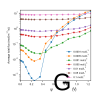
\includegraphics[width=0.5\linewidth]{img/SI-rect-reverse.pdf}
  \caption{Average total flux $J_{z}$ in the nanopore as
    a function of $\psi_{\mathrm{G}}$ at different concentrations. The
    range of $\psi_{\mathrm{G}}$ is larger than the experimentally
    achievable value. The rejection of flux becomes weaker after a
    certain level of $\psi_{\mathrm{G}}$ is reached. Further
    increasing the surface potential of graphene may even enhance the
    transportation of ions, which is similar to the cases of ionic
    transistors.}
  \label{fig:reverse}
\end{figure}


\begin{figure}[htbp]
  \centering
  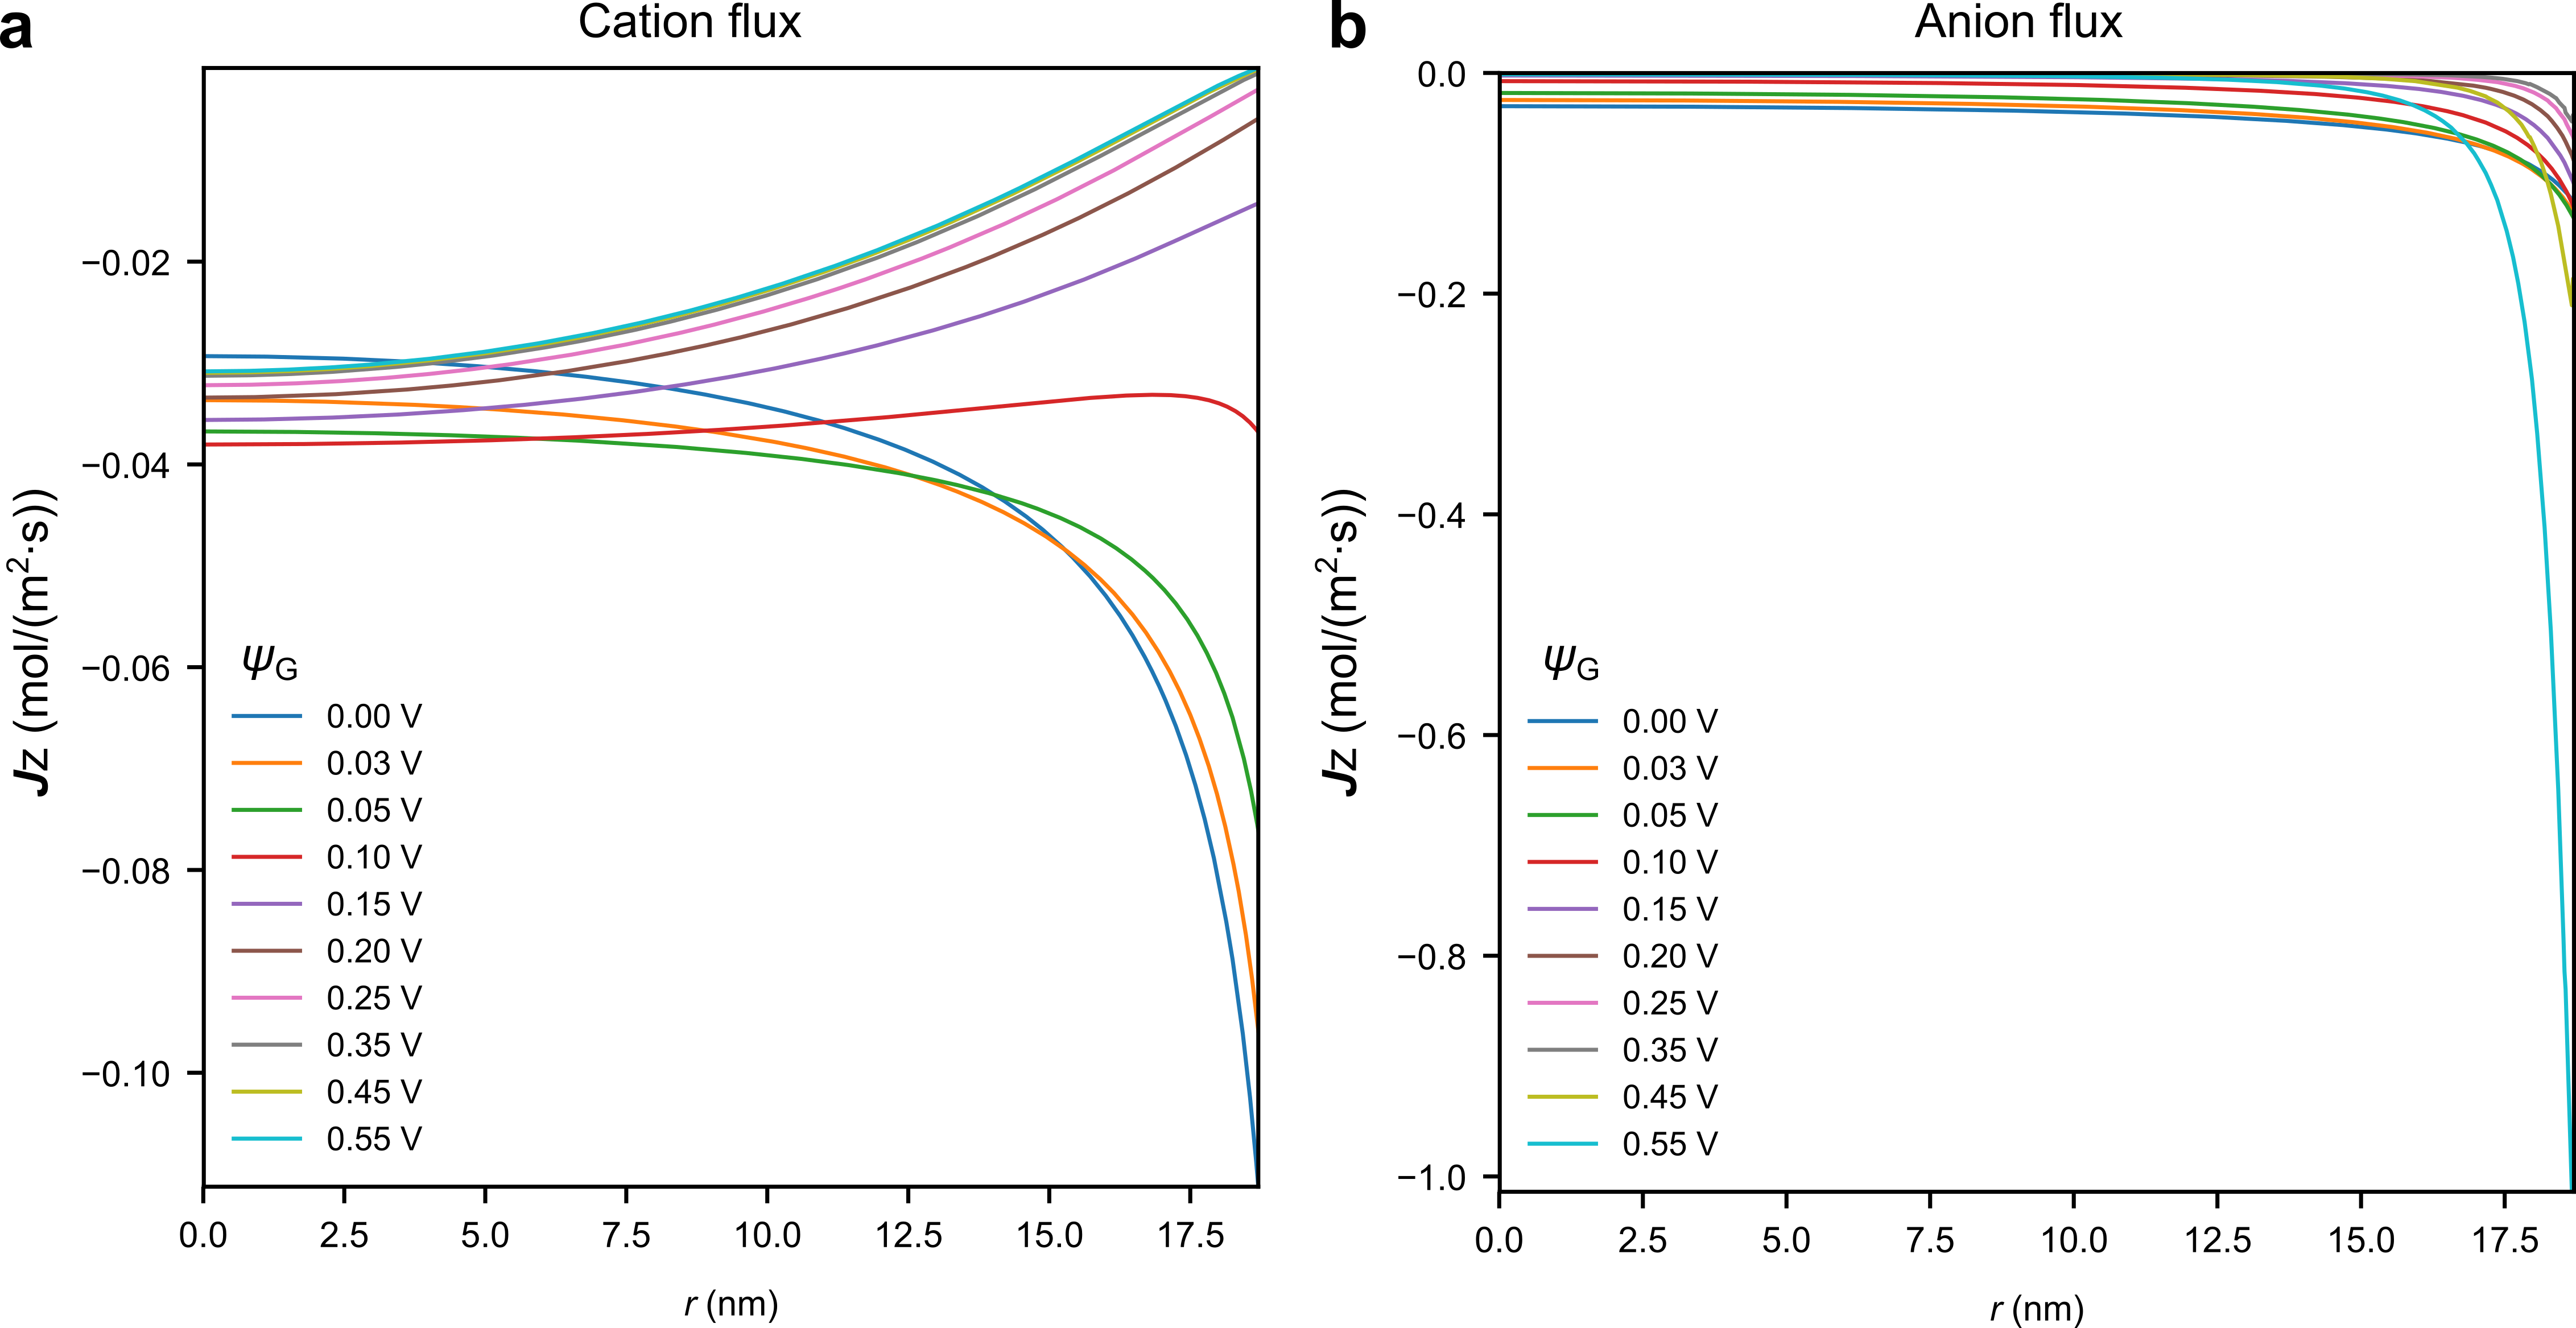
\includegraphics[width=0.8\linewidth]{img/SI-flux-larger.pdf}
  \caption{Spatial distribution of $J_{z}$ at $z = 0$ as a function
    of $r$ in a nanopore with $r_{\mathrm{G}}$ = 20 nm, at different
    levels of $\psi_{\mathrm{G}}$ (larger than experimentally
    achievable values) for cation (\textbf{a}.) and anion
    (\textbf{b}.). The cation flux becomes nearly saturated with
    increasing $\psi_{\mathrm{G}}$, while the flow of anion near the
    pore edge becomes much larger. The drastic increase of
    pore-bounded anion flux is caused by the accumulation of anions
    near the graphene surface, and in turn causes the increasing of
    total flux as seen in \Fig \ref{fig:reverse}.}
  \label{fig:large-V}
\end{figure}
\clearpage{}

\section{Effect of pore size distribution}
\label{sec:pore-dist}

In this section we provide a detailed discussion about the
influence of pore size distribution on the salt rejection through the
PG-PCTE membrane. Larger pores are the major contributors to salt flux, while at the same time, the effect of rejection is least pronounced.
As seen from main text Fig. \ref{fig:1}c
inset, the average distance between individual nanopores is larger
than the largest Debye length studied here ($\sim{}$ \unit[30]{nm} for 1 mM 1:1
salt solution), we can assume that the ionic transport pathways
through different nanopores do not influence each other and the total
ionic flux $\boldsymbol{J}_{\mathrm{PG}}$ is the summation of fluxes
through individual pores $\boldsymbol{J}_{i}$:
\begin{equation}
\label{eq:J-total}
\boldsymbol{J}_{\mathrm{PG}} = \sum_{i} \boldsymbol{J}_{i} = \sum_{r_{i}} x_{r_{i}} \boldsymbol{J}_{r_{i}}
\end{equation}
where $r_{i}$ is the radius of individual pores,
$\boldsymbol{J}_{r_{i}}$ and $x_{r_{i}}$ are the flux of individual
pore and the distribution probability when
$r_{\mathrm{G}} = r_{i}$. The salt rejection factor
$\xi$ through graphene is then expressed as:
\begin{equation}
  \label{eq:xi-pore}
  \begin{aligned}
    \xi &= 1 - \frac{\sum_{r_{i}} \boldsymbol{J}_{r_{i}} x_{r_{i}}}
           {\sum_{r_{i}} \boldsymbol{J}_{r_{i}}(V_{\mathrm{G}} = 0) x_{r_{i}}} \\
           &= 1 - \frac{\sum_{r_{i}} \hat{J}_{r_{i}} r_{i}^{2} x_{r_{i}}}
           {\sum_{r_{i}} \hat{J}_{r_{i}}^{0} r_{i}^{2} x_{r_{i}}} \\
           % &approx 1 - \sum_{r_{i}} \frac{\hat{J}_{r_{i}}}{\hat{J}_{r_{i}}^{0}}
           % \frac{r_{i}^{2} x_{r_{i}}} {\sum_{r_{i}} r_{i}^{2} x_{r_{i}}} \\
           &\approx \sum_{r_{i}} \left(1 -  \frac{\hat{J}_{r_{i}}}{\hat{J}_{r_{i}}^{0}}\right) w_{r_{i}} \\
           &= \sum_{r_{i}} \xi_{r_{i}} w_{r_{i}}
  \end{aligned}
\end{equation}
where $\hat{J}$ and $\hat{J}^{0}$ are the flux normalized by pore area
when $V_{\mathrm{G}} = 0$ and $V_{\mathrm{G}} \neq 0$, respectively,
$w_{r_{i}} = x_{r_{i}} r_{i}^{2} / \sum_{r_{i}} x_{r_{i}} r_{i}^{2}$ is
the contribution to the salt rejection from individual pore rejection
rate $\xi_{r_{i}}$. The linear combination between $\xi_{r_{i}}$ and
$\xi$ comes from the assumption that $\hat{J}^{0}$ is independent of
the pore size from the simple Ficknian diffusion.

To get an insight of the influence of the pore size distribution on
the salt rejection, we combine Equation \ref{eq:xi-pore} with main
text Fig. \ref{fig:5}b for the salt rejection of a 1:1
electrolyte to get the pore-distribution-related salt rejection, where
the pore distribution is taken from the SEM image of real samples (for
instance main text Fig. \ref{fig:1}c inset). Fig.
\ref{fig:simple-rect-pore}a shows the contribution $w$ and $\xi$ as
a function of $r_{\mathrm{G}}$ for individual pores when
$V_{\mathrm{G}}$ = 1.25 V. As can be seen, the majority of pores fall
within the regime of $\lambda_{\mathrm{D}} / r_{\mathrm{G}} > 1$,
corresponding to $\xi(r_{\mathrm{G}}) > 0.6$. As a result, considering
the pore distribution reduces the value of $\xi$ to $\sim{}$80\% to
that of a single 20 nm-diameter nanopore (Fig.
\ref{fig:simple-rect-pore}b), which is indeed close to the highest
$\xi$ values experimentally observed (for 1mM NaCl system). Such high
salt rejection even after considering the pore size distribution, can
be explained by the non-linear nature of $\xi$ with $r_{\mathrm{G}}$
and $V_{\mathrm{G}}$. As seen in main text Fig{} \ref{fig:5}b,
for large $V_{\mathrm{G}}$ and $\lambda_{\mathrm{D}} / r_{\mathrm{G}}$
regions, $\xi$ reaches a ``plateau'' with its value close to 1. For
the fabricated PG samples, most pores are within such region when
$V_{\mathrm{G}}$ = 1.25 V and $c_{0}$ = 0.1 mM, which gives a minor
change of $\xi$ despite the wide span of pore sizes. In other words,
although nanopores as large as 60 nm exist in the system, considerably
high salt rejection more than 80\% can still be achieved.

\begin{figure}[htbp]
  \centering
   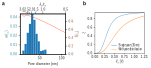
\includegraphics[width=0.9\linewidth]{img/SI-simple-pore-dist.pdf}
   \caption{Salt rejection after considering the pore size
     distribution. \textbf{a}. $w$ (left axis) and $\xi$ (right axis)
     as a function of $r_{\mathrm{G}}$ for the experimental pore size
     distribution with $c_{0}$ = 0.1 mM and $V_{\mathrm{G}}$ = 1.25 V.
     \textbf{b}. Salt rejection ratio $\xi$ as a function of $V_{\mathrm{G}}$ of a
     0.1mM 1:1 salt from a 20 nm-diameter nanopore (blue line) and
     from the experimental pore size distribution (orange line), by
     applying Equation \ref{eq:xi-pore} to main text Fig.
     \ref{fig:5}b.}
  \label{fig:simple-rect-pore}
\end{figure}

To include the pore size distribution effect for all the salts
studied, we performed FEM analysis for the salt rejection through
single nanopore of different salts with $r_{\mathrm{G}}$ ranges from
2.5 nm to 35 nm, while keeping $c_{0}$ constant at 0.1 mM. As shown in
Fig. \ref{fig:xi-salts-pore}, the behavior of $\xi$ vary with the
type of salt. As expected, the overall $\xi$ for monovalent salts
(KCl, NaCl, LiCl) is larger than multivalent salts due to the longer
Debye length. Moreover, $\xi$ of monovalent salts varies less with the
pore size compared with multivalent salts. This can be explained by
the non-linear dependency of $\xi$ on
$\lambda_{\mathrm{D}} / r_{\mathrm{G}}$ as discussed above. Combine
the FEM-simulated $\xi$ values with the experimental pore size
distribution, we obtain main text Fig. \ref{fig:6}.

\begin{figure}[htbp]
  \centering
   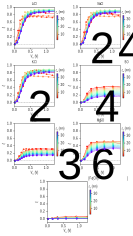
\includegraphics[width=0.75\linewidth]{img/SI-xi-salt-pore-size.pdf}
  \caption{FEM-simulated salt rejection ratio $\xi$ as a function of
    $V_{\mathrm{G}}$ through single nanopores for different salts with
    varied pore radius. All salts have concentration $c_{0}$ = 0.1 mM.}
  \label{fig:xi-salts-pore}
\end{figure}


\pagebreak
\section{Further details of the numerical simulation }
\label{sec:numer}

The numerical simulations were carried out using COMSOL Multiphysics
5.3a. The simulation domain is shown in \Fig \ref{fig:scheme}. To
simplify the geometry, we use axial symmetric coordinate system. The
radius \textit{L} and height \textit{H} of both HCR and LCR are set to
20 $r_{\mathrm{G}}$, the radius of the nanopore. The potential at the
bottom of the LCR and the center of the graphene domains are set to be
0 and $\psi_{\mathrm{G}}$, respectively. The potential at the end of
HCR is not set explicitly, but rather determined through the Poisson
equation with no flux boundary condition
$\boldsymbol{D}^{\mathrm{norm}}=0$. The relative permittivity in the
HCR and LCR is set as $\varepsilon_{\mathrm{}}=78$. The relative
permittivity of the Stern layer is set to
$\varepsilon_{\mathrm{H}}=20$\cite{Conway_1951} and for the graphene
domain we set the relative permittivity as a large number
(e.g. $10^{5}$) for a better convergence of the solver.  For the
transport of diluted ionic species, we use the PNP equations, to
describe the diffusion and drift of the ions, which can be further
unified by the gradient of electrochemical potential, as described in
the main text. The initial values of the electrolyte is set to $c_{0}$
in HCR and 0.1 $c_{0}$ in LCR. At the ends of the cells in the
z-direction, we use the inlet boundaries conditions for the
concentration of electrolytes, that the concentration on these
boundaries remains the same with the initial value, due to the
effective mixing in the experimental setup.

\begin{figure}[htbp]
  \centering
  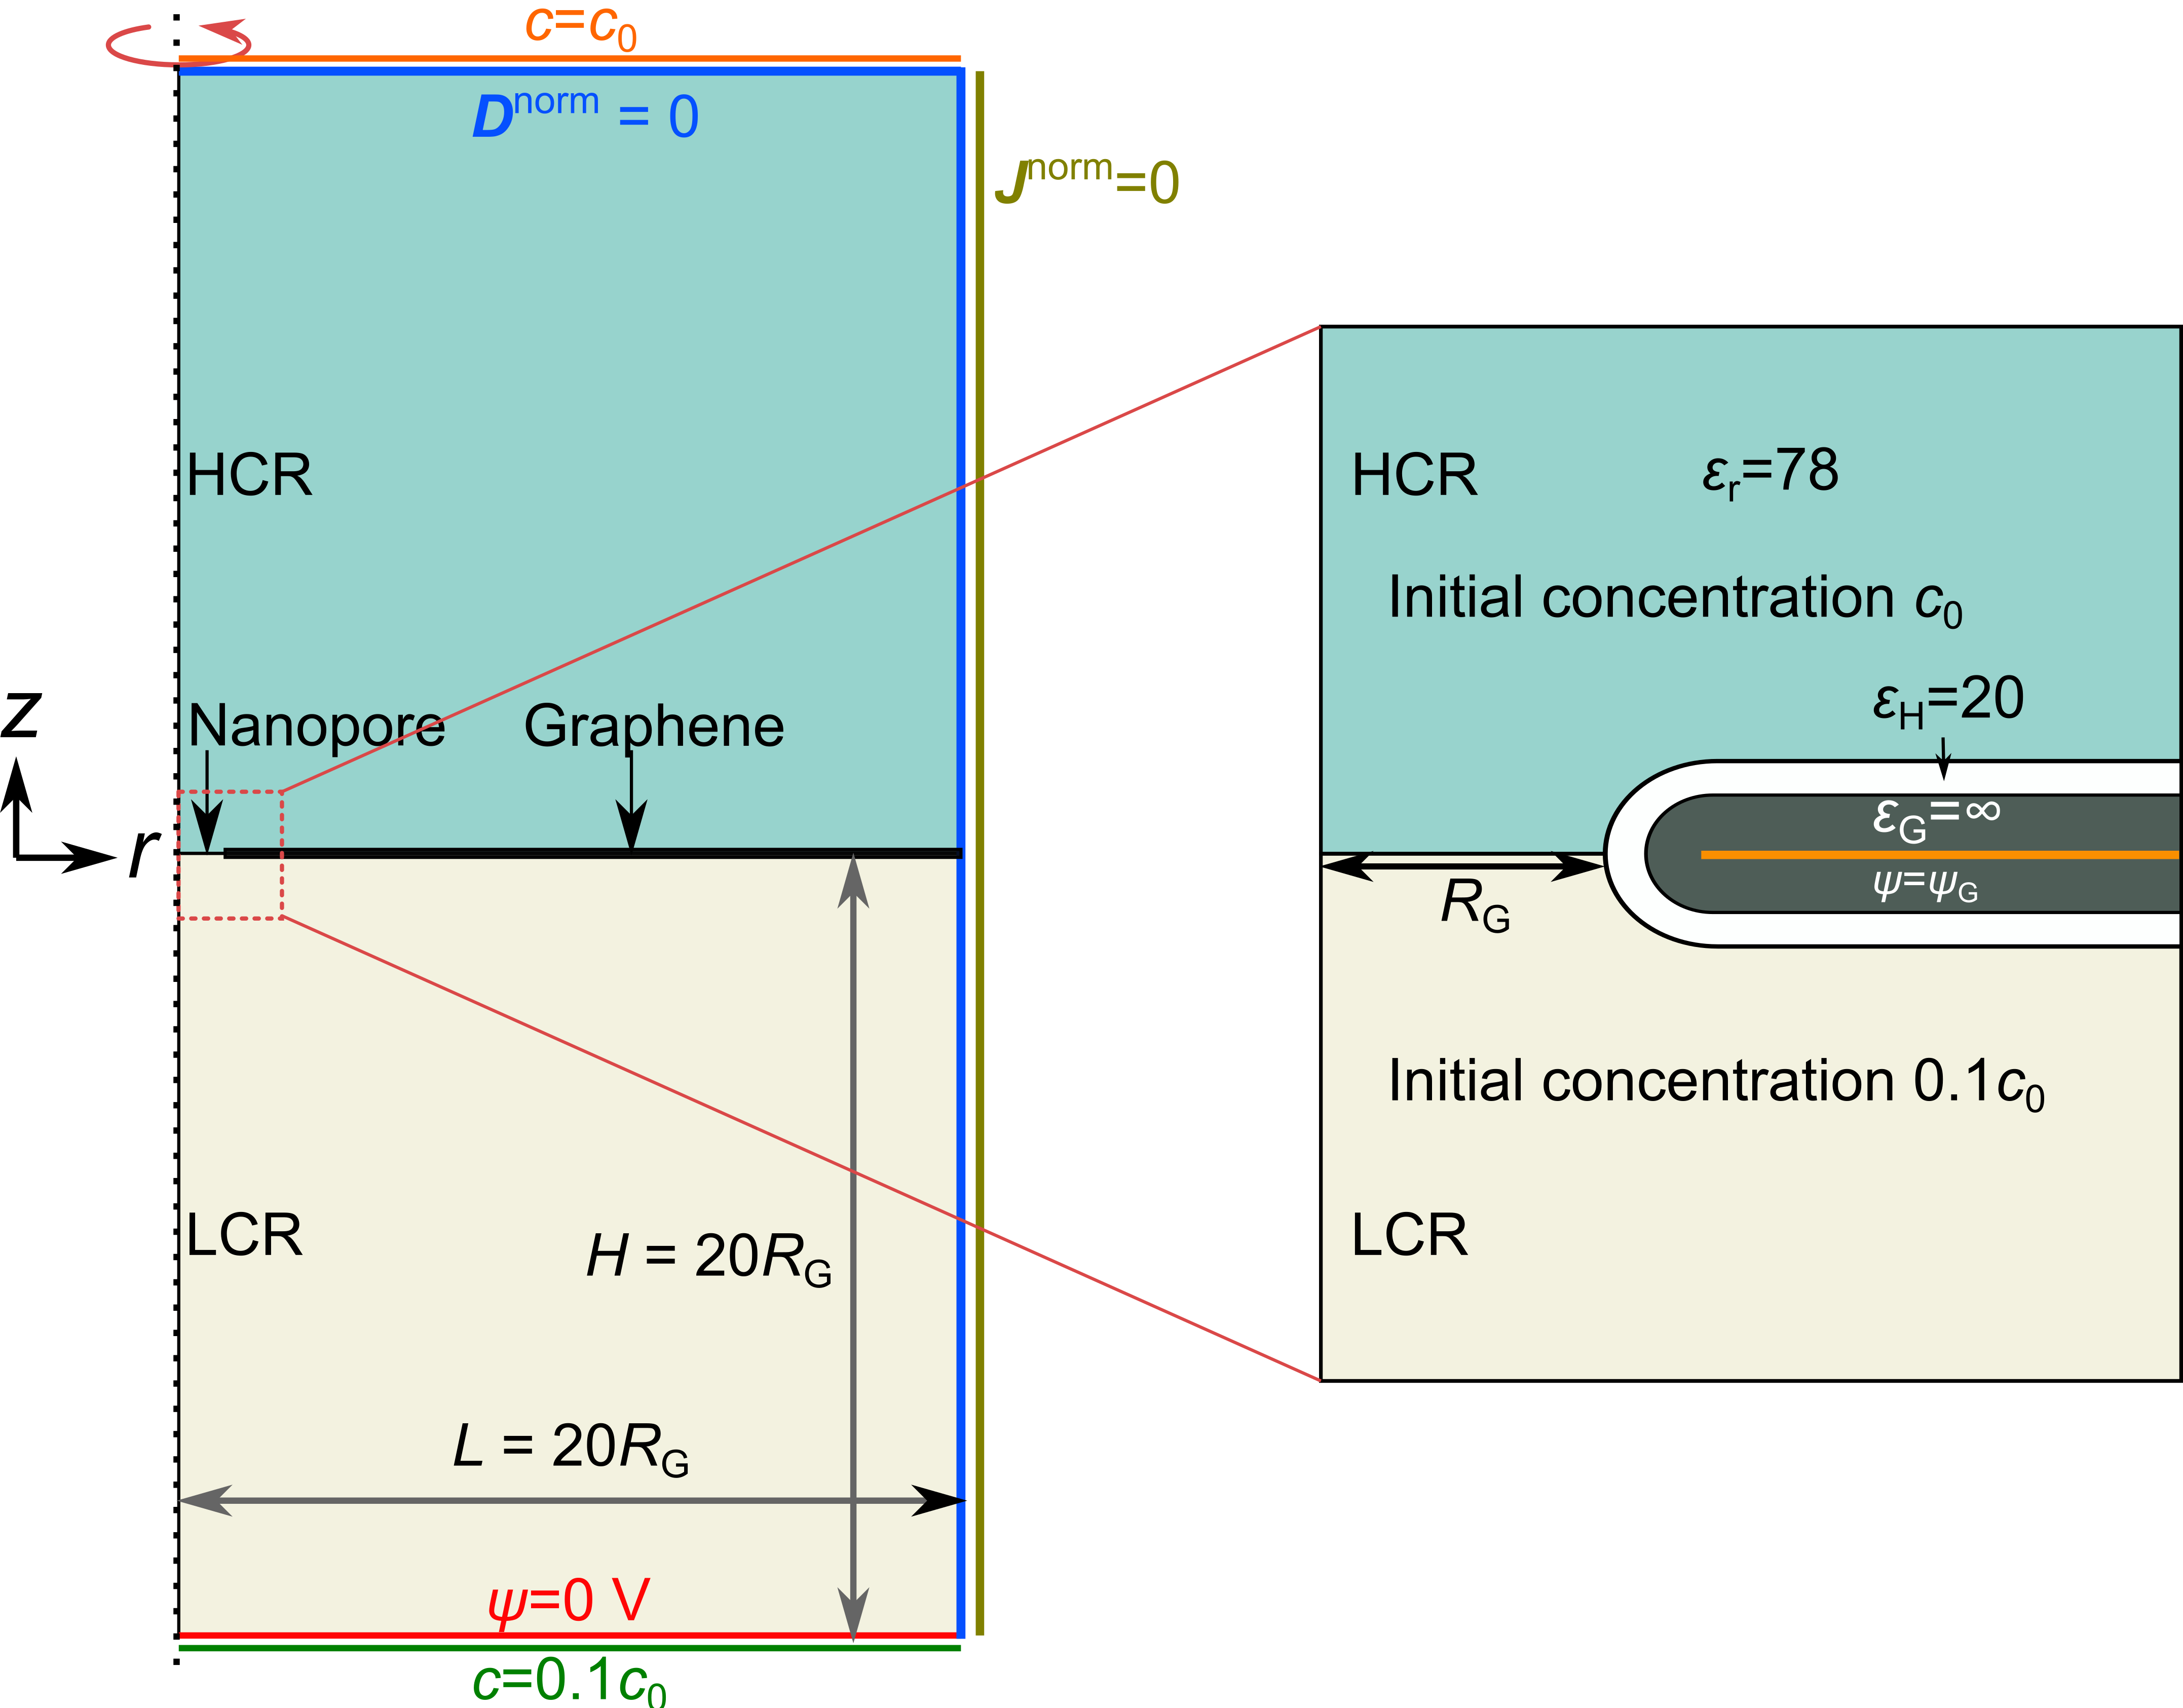
\includegraphics[width=0.8\linewidth]{img/SI-numerical-1.png}
  \caption{Scheme of the simulation domain used. Left: geometry of the
    whole simulation domain. Right: configuration near the graphene
    nanopore, corresponding to the red rectangle on the left side.}
  \label{fig:scheme}
\end{figure}

The transport of ionic species is described by the steady-state
Nernst-Planck equation:
\begin{eqnarray}
  \label{eq:pnp}
  \nabla \cdot \boldsymbol{J}_{i} = -\nabla \cdot \left( \frac{D_{i}}{k_{\mathrm{B}}T} c_{i} N_{\mathrm{A}} \nabla \mu_{i}\right)
  = -\nabla \cdot \left( \frac{D_{i}}{k_{\mathrm{B}} T} c_{i} N_{\mathrm{A}}
  [k_{\mathrm{B}}T \nabla \ln x_{i} + z_{i} e \nabla \psi]\right) = 0\\
  x_{i} = \frac{c_{i}}{\sum_{i} c_{i} + c_{\mathrm{H_{2}O}}}
\end{eqnarray}
The potential distribution within the whole simulation domain is
described by the Poisson equation:
\begin{equation}
  \label{eq:poisson}
  \nabla \cdot (\varepsilon_{\mathrm{m}} \varepsilon_{0} \nabla \psi) = -N_{\mathrm{A}} e \sum_{i} c_{i}z_{i}
\end{equation}
Where $\varepsilon_{\mathrm{m}}$ is the relative permittivity of
domain m. The contribution of mobile charges is only valid in the
solution domain. The use of a large $\varepsilon_{\mathrm{G}}$ ensures
that the potential in the whole simulation domain can be solved
continuously. 

To simulate the applied external bias $V_{\mathrm{G}}$, we set the
value of $\psi_{\mathrm{G}}$ explicitly and extract the charge
$\sigma_{\mathrm{G}}$ by:
\begin{equation}
  \label{eq:sigma-G}
  \sigma_{\mathrm{G}} = - {\displaystyle \frac{\int_{\mathrm{\Omega}} z_{i} c_{i} N_{\mathrm{A}} e \mathrm{d}^{3} \Omega}{S_{\mathrm{G}}}}
\end{equation}
and $V_{\mathrm{G}}$ is then calculated by:
\begin{eqnarray}
  \label{eq:VG}
  V_{\mathrm{G}} = \Delta \phi_{\mathrm{G}} + \psi_{\mathrm{G}}\\
  \sigma_{\mathrm{G}} = \int_{0}^{\Delta \phi_{\mathrm{G}}} \frac{1}{C_{\mathrm{Q}}(\phi_{\mathrm{G}})} \mathrm{d} \phi_{\mathrm{G}}
\end{eqnarray}
where the quantum capacitance
$C_{\mathrm{Q}}=\partial \sigma_{\mathrm{G}}/\partial
\phi_{\mathrm{G}}$ is calculated by Eq. 8 in main text.

\begin{figure}[htbp]
  \centering
  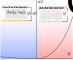
\includegraphics[width=0.5\linewidth]{img/SI-trap.png}
  \caption{Schematic illustration of the origin of the asymmetric
    rejection with respect to $V_{\mathrm{G}}$. Due to the
    existence of surface charge traps at negative $V_{\mathrm{G}}$,
    the graphene is less charged compared to the positive
    $V_{\mathrm{G}}$.}
  \label{fig:trap}
\end{figure}

Note that due to the existence of electron traps on graphene due to
fabrication process, the induced charge traps on graphene effectively
reduce the charge density on graphene and greatly attenuate the
surface potential on graphene, as illustrated in Fig. \ref{fig:trap}. This effect is universally observed in
CVD-graphene-based field effect transistors in air, while the
mechanism is fully understood yet. In view of this, we only simulate
the situation where $V_{\mathrm{G}}>$ 0 for the salt rejection
mechanism. The trend that $\xi$ is almost independent of
$V_{\mathrm{G}}$ when $V_{\mathrm{G}}<$ 0 can be qualitatively
explained by the existence of surface charge traps as stated above.
We have also tested the mesh-independence of our solutions. As show in
in Fig. \ref{fig:mesh}a, we use two parameters to control the
refinement of the mesh entities: (i) triangle mesh division
$N_{\mathrm{div}}$, giving the smallest triangle mesh size
$\delta_{\mathrm{G}} / N_{\mathrm{div}}$, where $\delta_{\mathrm{G}}$
is the thickness of graphene, and (ii) division of mesh
$N_{\mathrm{b}}$, on the boundary $0<r<r_{\mathrm{G}};z=0$. The
solution convergence is evaluated by the mean absolute error (MAE) of
anion flux $\boldsymbol{J}_{z}$ on the boundary
$0<r<r_{\mathrm{G}};z=0$, as shown in Fig.
\ref{fig:mesh}b. The solution of the PNP model is sensitive to the
value $N_{\mathrm{b}}$, and can be regarded numerically converged when
$N_{\mathrm{b}}>100$. Combining the calculation effort and numerical
precision, we adapt the value $N_{\mathrm{div}}=5$ and
$N_{\mathrm{b}}=100$ in our simulations.

\begin{figure}[htbp]
  \centering
  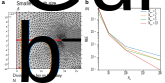
\includegraphics[width=0.8\linewidth]{img/SI-mesh.pdf}
  \caption{Mesh independence of the solution. \textbf{a}. Scheme of
    the mesh refinement near the graphene pore. The values
    $N_{\mathrm{div}}$ and $N_{\mathrm{b}}$ controls the size of mesh
    along the boundary $z=0, 0<r<r_{\mathrm{G}}$ (shown in
    red). \textbf{b}. Mean absolute error (MAE) of the anion flux
    $\boldsymbol{J}_{z}$ along the boundary $z=0,
    0<r<r_{\mathrm{G}}$. The error is more sensitive to
    $N_{\mathrm{b}}$ than $N_{\mathrm{div}}$.}
  \label{fig:mesh}
\end{figure}

\section{Conductivity and Debye length for all salts}
\label{sec:salts}
In Table \ref{tab:conductivity}, the conductivities and calculated Debye
lengths for 6 salts are shown. At the same concentration, the higher
ionic strength of the multivalent salts leads to a reduction of the
respective Debye lengths.

\begin{table}[htbp]
  \centering
  \begin{tabular}{lcc}
    \hline
    Solution & Conductivity (mS$\cdot$cm$^{-1}$) & $\lambda_{\mathrm{D}}$ (nm) \\
    \hline
    0.1 mM NaCl &1.80$\times$10$^{-2}$  &30.4\\
    0.1 mM LiCl &1.58$\times$10$^{-2}$ &30.4\\
    0.1 mM CaCl$_{2}$&  2.19$\times$10$^{-2}$ &17.2\\
    0.1 mM MgSO$_{4}$   &3.27$\times$10$^{-2}$ &15.2\\
    0.1 mM K$_{2}$SO$_{4}$      &4.16$\times$10$^{-2}$ &17.2\\
    0.1 mM K$_{3}$[Fe(CN)$_{6}$]&       5.95$\times$10$^{-2}$  &12.4\\
    \hline
  \end{tabular}
  \caption{Conductivity and $\lambda_{\mathrm{D}}$ of various salts.}
  \label{tab:conductivity}
\end{table}




\end{document}
